\chapter{Metodolog\'ia}
\label{ch:metodologia}

El Cap\'itulo~\ref{ch:marco} construy\'o el aparato formal que sustenta la arquitectura predictiva: sistemas de rating din\'amico, modelos de conteo, integraci\'on de covariables ex\'ogenas y m\'etricas de evaluaci\'on. El presente cap\'itulo transita de la teor\'ia a la operacionalizaci\'on. Se describe, de manera lineal, c\'omo se recolectaron y procesaron los datos (Secci\'on~\ref{sec:fuentes}), c\'omo se construyeron los \'indices compuestos y se seleccionaron las covariables ex\'ogenas (Secciones~\ref{sec:procesamiento} y~\ref{sec:seleccion_covariables}), y c\'omo se implement\'o, entren\'o y calibr\'o cada bloque funcional del sistema en cascada (Secciones~\ref{sec:arquitectura} a~\ref{sec:metricas_eval}). Los resultados num\'ericos de los experimentos se reservan para el cap\'itulo siguiente, de modo que este cap\'itulo funcione como manual de replicaci\'on del proceso de inferencia.

% ============================================================
% SECCION 3.1 -- Fuentes de datos
% ============================================================

\section{Fuentes de datos}
\label{sec:fuentes}

El presente estudio integra informaci\'on proveniente de cinco fuentes principales, seleccionadas por su cobertura temporal, granularidad y confiabilidad en los dominios deportivo, econ\'omico, ambiental e institucional. La estrategia de recolecci\'on combina extracci\'on automatizada v\'ia \textit{web scraping}, consultas a APIs abiertas y transcripci\'on manual de portales especializados. A continuaci\'on se describe cada fuente, el periodo cubierto, las variables recopiladas y las restricciones t\'ecnicas que condicionaron su operacionalizaci\'on.

\subsection{Datos deportivos}
\label{subsec:fbref}

La fuente de datos de rendimiento fue el sitio FBRef.com \cite{FBRef}, especializado en estad\'isticas hist\'oricas de f\'utbol. Se recopilaron datos correspondientes al per\'iodo 1 de enero de 2017 al 31 de diciembre de 2025, abarcando 25 competiciones distribuidas en cuatro confederaciones continentales y un torneo global:

\begin{itemize}
	\item \textbf{Europa:} Premier League (Inglaterra), LaLiga (Espa\~na), Bundesliga (Alemania), Serie A (Italia), Ligue 1 (Francia), Super League (Grecia), UEFA Champions League, UEFA Europa League, UEFA Conference League.
	\item \textbf{Norteam\'erica, Centroam\'erica y el Caribe:} Major League Soccer (Estados Unidos), Liga MX (M\'exico), CONCACAF Champions League.
	\item \textbf{Suram\'erica:} Liga Profesional / Superliga (Argentina), Brasileir\~ao (Brasil), Liga FutVe (Venezuela), Copa Libertadores, Copa Sudamericana.
	\item \textbf{Asia:} J1 League (Jap\'on), K League 1 (Corea del Sur), Saudi Pro League (Arabia Saudita), Persian Gulf Pro League (Ir\'an), AFC Champions League Elite, AFC Champions League Two.
	\item \textbf{Intercontinental:} FIFA Club World Cup.
\end{itemize}

La selecci\'on responde a un criterio de cobertura: las principales ligas nacionales de cuatro confederaciones con datos completos en FBRef para el per\'iodo analizado, m\'as los torneos continentales e intercontinentales asociados. La extracci\'on se realiz\'o mediante un sistema de \textit{web scraping} desarrollado en Python, implementado en los \textit{scripts} \texttt{ScrapperV4a.py}, \texttt{ScrapperV4b.py} y  \texttt{ScrapperV4c.py}, que operan de manera coordinada sobre el mismo esquema de datos. El proceso se organiza en cinco etapas que se  describen a continuaci\'on.

\paragraph{Navegaci\'on por \'indice diario.} Para cada fecha en el rango de estudio se construye la URL del \'indice diario (\texttt{fbref.com/en/matches/YYYY-MM-DD}) y se realiza una petici\'on HTTP sobre una sesi\'on configurada con \texttt{curl\_cffi}, que impersona la huella TLS de un navegador Chrome. En caso de indisponibilidad de esta biblioteca, el sistema recurre a \texttt{cloudscraper} o a \texttt{requests} est\'andar como \textit{fallbacks}.

\paragraph{Detecci\'on y evasi\'on de bloqueos.} Si la respuesta contiene c\'odigos de estado 403 o 429, o si el HTML corresponde a una p\'agina de desaf\'io de Cloudflare, se activa un mecanismo de \textit{warm-up} basado en Selenium con Microsoft Edge, en un perfil temporal y sin modo \textit{headless}. Una vez superado el desaf\'io, las cookies obtenidas se transfieren a la sesi\'on HTTP principal y se persisten en disco (\texttt{fbref\_cookies.json}) para su reutilizaci\'on en ejecuciones posteriores. Este enfoque h\'ibrido reduce dr\'asticamente la frecuencia de intervenci\'on manual.

\paragraph{Filtrado por competici\'on.} Las p\'aginas de \'indice contienen tablas agrupadas por competici\'on. El sistema analiza el texto del elemento \texttt{<caption>} de cada tabla, lo normaliza (sin tildes, en min\'usculas) y lo compara contra una lista de patrones predefinidos. Las competiciones no deseadas se descartan mediante una lista de exclusi\'on que filtra, entre otras, divisiones de ascenso, torneos juveniles y ligas no incluidas en el estudio. Para cada fila de las tablas seleccionadas se extraen: fecha del partido, nombre de la competici\'on, equipo local, equipo visitante, marcador, identificador \'unico del partido y URL de la p\'agina detallada.

\paragraph{Control de frecuencia.} Para minimizar el riesgo de bloqueo y distribuir la carga a lo largo de la ejecuci\'on, se  implement\'o un \textit{rate limiting} global que impone un espaciado m\'inimo entre peticiones y una cota de peticiones por ventana temporal.

\paragraph{Descarga de estad\'isticas detalladas.} Para cada partido identificado, el sistema descarga la p\'agina detallada y extrae las tablas de estad\'isticas individuales por jugador (identificadores que comienzan con \texttt{stats\_}) y las tablas agregadas de equipo (\texttt{summary}). Muchas de estas tablas est\'an anidadas dentro de comentarios HTML, por lo que el \textit{parser}, construido sobre \texttt{BeautifulSoup}, procesa tanto elementos visibles como comentados. Los datos se organizan en un esquema com\'un y se exportan en formato CSV por tabla, junto con un archivo de manifiesto que verifica la completitud de cada descarga.

Adicionalmente a la extracci\'on automatizada, se incorporaron manualmente 181 partidos que no existen originalmente en las p\'aginas \'indice de FBRef: 28 de la CONCACAF Champions Cup, 151 de la AFC Champions League Elite y 2 de la AFC Champions League Two. Estos registros se transcribieron al mismo esquema del conjunto de datos maestro y se concatenaron verticalmente, garantizando la alineaci\'on exacta de columnas. Las dos competiciones asi\'aticas constituyen el \'unico bloque del universo cuya totalidad de partidos no proviene del \textit{scraper}; en el caso de la CONCACAF Champions Cup, la incorporaci\'on manual cubre \'unicamente las ediciones previas a su disponibilidad en FBRef.

Una vez recolectadas las p\'aginas detalladas de cada partido, el \textit{pipeline} opera directamente sobre las tablas de estad\'isticas individuales por jugador extra\'idas de cada archivo, sin pasar por una consolidaci\'on intermedia en un \'unico archivo maestro. El identificador \texttt{match\_id} proviene directamente del slug del URL de la p\'agina del partido en FBRef; no se computa localmente. Sobre esa base se construye una clave derivada \texttt{match\_id\_new} con formato
\begin{equation}
	\texttt{match\_id\_new} = \texttt{YYYYMMDD}\_\texttt{home\_team\_id}\_\texttt{away\_team\_id},
	\label{eq:match_id_new}
\end{equation}

donde la fecha se extrae del campo \texttt{match\_date} y se codifica como \texttt{YYYYMMDD}, y cada identificador de equipo (\texttt{home\_team\_id} y \texttt{away\_team\_id}) es una cadena hexadecimal de ocho caracteres, tomada del atributo \texttt{href} que FBRef embebe en las tablas de cada p\'agina de partido; cada bloque se separa con guiones bajos. Esta clave, junto con las columnas \texttt{home\_team} y  \texttt{away\_team}, sirve como ancla para todas las uniones posteriores del \textit{pipeline} y es la unidad de observaci\'on que atraviesa las fases de procesamiento, integraci\'on de covariables y entrenamiento.

Cada archivo descargado para un equipo y partido contiene, adem\'as de los metadatos del encuentro, la informaci\'on desagregada por jugador y una fila consolidada. Los metadatos invariantes extra\'idos son: fecha, competici\'on, nombre normalizado del equipo e identificador hexadecimal del equipo. A nivel de jugador, se capturan el dorsal, la nacionalidad, la posici\'on espec\'ifica en  ese partido y la edad expresada en a\~nos y d\'ias. Las m\'etricas deportivas de acumulaci\'on, que constituyen el insumo central del an\'alisis, son: minutos jugados (\texttt{min}), goles (\texttt{goals}), asistencias (\texttt{assist}), penales  marcados (\texttt{goalspen}), penales intentados (\texttt{attpen}), tiros totales (\texttt{shots}), tiros a puerta (\texttt{shtarget}), tarjetas amarillas (\texttt{yellowcard}), tarjetas rojas  (\texttt{redcard}), faltas cometidas (\texttt{fouls}), faltas recibidas (\texttt{foulsd}), fueras de juego (\texttt{offside}), centros (\texttt{crosses}), entradas ganadas (\texttt{tacklesw}), intercepciones (\texttt{interceptions}), autogoles (\texttt{owngoal}), penales ganados (\texttt{penkickgen}) y penales concedidos (\texttt{penkickcon}).

\subsection{Datos econ\'omicos}
\label{subsec:transfermarkt}
\label{subsec:datosmacro}

Los datos econ\'omicos se obtuvieron en dos escalas complementarias. A nivel de club se utiliz\'o la plataforma Transfermarkt \cite{Transfermarkt}; a nivel de pa\'is se recurri\'o al portal Datosmacro \cite{Datosmacro}, perteneciente al diario Expansi\'on.

\paragraph{Nivel de club (micro).} 

Dado que este sitio implementa medidas que impiden el \textit{scraping} automatizado, la recopilaci\'on se realiz\'o de forma manual, transcribiendo la informaci\'on directamente desde el sitio web a archivos de hoja de c\'alculo. Se extrajeron los siguientes campos para cada club, con periodicidad semestral coincidiendo con los cierres de los mercados de fichajes de verano e invierno:

\begin{itemize}
	\item Valor total de mercado de la plantilla (en millones de euros).
	\item N\'umero total de jugadores inscritos.
	\item Cantidad de jugadores extranjeros (cuya nacionalidad no corresponde al pa\'is de la liga).
	\item Ingresos por venta de jugadores (en millones de euros) por ventana de fichajes.
	\item Gastos por compra de jugadores (en millones de euros) por ventana de fichajes.
\end{itemize}

A partir de estas variables se calcula el indicador derivado \textit{net spending}, detallado en la Secci\'on~\ref{subsec:integracion}.

\paragraph{Nivel de pa\'is (macro).} El portal Datosmacro recopila indicadores econ\'omicos oficiales de fuentes como el Banco Mundial, el Fondo Monetario Internacional y los institutos nacionales de estad\'istica. Los datos, de periodicidad anual, fueron transcritos manualmente a una hoja de c\'alculo para los quince pa\'ises incluidos inicialmente en el estudio. Las variables recopiladas son: Producto Interno Bruto (PIB, en millones de euros), tasa de inflaci\'on (porcentaje anual), Inversi\'on Extranjera Directa (IED, en millones de euros), poblaci\'on (en millones de habitantes), \'indice de Gini, gasto p\'ublico (en millones de euros) y deuda externa (en millones de euros).

\subsection{Datos meteorol\'ogicos y geogr\'aficos}
\label{subsec:openmeteo}
\label{subsec:estadios}

Las covariables ambientales y geogr\'aficas se construyeron a partir de dos fuentes complementarias: la API hist\'orica de Open-Meteo \cite{OpenMeteo} para las condiciones clim\'aticas, y una tabla maestra de estadios para la altitud, las coordenadas geogr\'aficas y la asistencia promedio.

\paragraph{Datos meteorol\'ogicos.} Los datos clim\'aticos asociados a cada partido se obtuvieron a trav\'es de la API hist\'orica de Open-Meteo \cite{OpenMeteo}. Dado que la plataforma impone un l\'imite de 9\,000 peticiones diarias, se opt\'o por una estrategia de muestreo mensual inspirada en la metodolog\'ia de Van Putten \cite{VanPutten2023}, quien emplea un enfoque similar para vincular condiciones clim\'aticas con resultados deportivos.

Para cada estadio se dispone de sus coordenadas geogr\'aficas (latitud y longitud), obtenidas manualmente mediante Google Maps. Se consulta la API de Open-Meteo para el d\'ia 15 de cada mes en el rango de estudio, a las 18:00 hora local, horario seleccionado por ser el m\'as frecuente de inicio de los partidos en las ligas analizadas. Las variables solicitadas son temperatura a 2 metros del suelo (en grados Celsius), humedad relativa a 2 metros del suelo (en porcentaje) y presi\'on atmosf\'erica a nivel del suelo (en hPa). A partir de la temperatura y la humedad relativa se computa la presi\'on de vapor de agua $P_{\mathrm{H_2O}}$ (en hPa) mediante la f\'ormula de Magnus:
\begin{equation}
	P_{\mathrm{H_2O}} = 6{.}112 \cdot 
	\exp\!\left(\frac{17{.}67 \cdot T}{T + 243{.}5}\right) \cdot 
	\frac{\mathrm{RH}}{100},
	\label{eq:magnus}
\end{equation}
donde $T$ es la temperatura en grados Celsius y $\mathrm{RH}$ la humedad relativa.

El protocolo resultante realiza una petici\'on por estadio al rango completo de fechas, extrayendo de cada respuesta los valores correspondientes al d\'ia 15 de cada mes. Esta estrategia mantiene el n\'umero total de consultas a la API dentro del l\'imite diario de 9\,000 peticiones, en contraste con un esquema alternativo que habr\'ia requerido una consulta individual por partido sobre los 37\,819 encuentros registrados tras la limpieza detallada en la Secci\'on~\ref{sec:procesamiento}. Durante el procesamiento posterior, a cada partido se le asocia el valor clim\'atico del mes correspondiente (Secci\'on~\ref{subsec:integracion}), asumiendo estabilidad intramensual de las condiciones meteorol\'ogicas en la sede del encuentro.

\paragraph{Datos de estadios.} Se construy\'o una tabla maestra de 437 estadios con informaci\'on de todos los clubes incluidos en el estudio, de los cuales 422 fueron efectivamente consultados en la API clim\'atica; los quince restantes corresponden a sedes neutrales codificadas pero nunca utilizadas en el panel final. Las fuentes utilizadas fueron Wikipedia (capacidad y ciudad, contrastada con Transfermarkt), Wikipedia y consultas espec\'ificas (altitud, en particular para estadios de alta monta\~na), Google Maps (coordenadas geogr\'aficas) y Transfermarkt \cite{Transfermarkt} (asistencia promedio anual). Esta tabla incluye los siguientes campos para cada estadio: identificador \'unico (\texttt{stadium\_id}), nombre oficial, ciudad, capacidad, altitud (metros sobre el nivel del mar), latitud, longitud y asistencia promedio por temporada (columnas \texttt{Assist\_\{temporada\}}).

Con la integraci\'on de estas cinco fuentes queda definido el cuerpo emp\'irico del trabajo. A partir de su procesamiento conjunto se derivan tres conjuntos de datos diferenciados por su ventana temporal y su riqueza de covariables, cuya generaci\'on y descripci\'on detallada se presentan en la Secci\'on~\ref{subsec:datasets_finales}.

% ============================================================
% SECCION 3.2 -- Procesamiento y limpieza de datos
% ============================================================

\section{Procesamiento y limpieza de datos}
\label{sec:procesamiento}

Una vez recolectados los datos crudos descritos en la Secci\'on~\ref{sec:fuentes}, se ejecut\'o un \textit{pipeline} de procesamiento cuyo objetivo es transformar registros dispersos y heterog\'eneos en un panel estructurado listo para la inferencia. El flujo de trabajo se implement\'o en Python sobre las bibliotecas \texttt{pandas}, \texttt{numpy} y \texttt{scikit-learn}, y se organiza en seis etapas: consolidaci\'on y aplanamiento de las estad\'isticas deportivas; depuraci\'on y control de calidad del universo de equipos; integraci\'on horizontal de variables clim\'aticas, de estadio y econ\'omicas; construcci\'on de m\'etricas compuestas y promedios m\'oviles; filtrado temporal y por competici\'on e imputaci\'on de valores faltantes y estandarizaci\'on; y generaci\'on de los conjuntos de datos finales.

\subsection{Consolidaci\'on y aplanamiento de registros deportivos}
\label{subsec:aplanamiento}

Los archivos extra\'idos de FBRef mediante los \textit{scripts} de \textit{scraping} (Secci\'on~\ref{subsec:fbref}) se depositan en lotes anuales. En total se procesaron 108\,766 archivos \texttt{summary} correspondientes a las 25 competiciones listadas en la Secci\'on~\ref{subsec:fbref}. Cada archivo contiene, para un partido y un equipo, una fila por jugador y una fila consolidada al final. El primer paso del \textit{pipeline} consiste en consolidar estos fragmentos en un \'unico \texttt{DataFrame} y aplanar la estructura a nivel de equipo-partido.

\paragraph{Normalizaci\'on de esquemas.} La estructura de columnas var\'ia ligeramente entre temporadas debido a la aparici\'on de nuevas m\'etricas o a renombramientos en la fuente. Se recolecta el conjunto universal de columnas y se fuerza un esquema homog\'eneo: a cada archivo anual se le a\~naden las columnas faltantes con valores nulos, garantizando la concatenabilidad vertical. Posteriormente se renombran las columnas al esquema interno del \textit{pipeline} mediante un diccionario de mapeo que traduce etiquetas multinivel como \texttt{Performance~Gls} o \texttt{Performance~SoT} a identificadores planos (\texttt{Goals}, \texttt{ShTarget}, etc.). Tras el aplanamiento se obtuvieron 98\,972 filas con \texttt{match\_id\_new} v\'alido; todas ellas conservaron la informaci\'on de fecha necesaria para el resto del \textit{pipeline}.

\paragraph{Aplanamiento y agregaci\'on.} Para cada archivo correspondiente a un partido y un equipo, la agregaci\'on de las m\'etricas num\'ericas de jugadores satisface formalmente
\begin{equation}
	\text{team\_stats}(m,t) = \sum_{j \in \text{jugadores}(m,t)} 
	\text{player\_stats}_j,
\end{equation}
donde $m$ indexa el partido y $t$ el equipo. Si bien esta sumatoria define conceptualmente las estad\'isticas agregadas, cada archivo contiene en su \'ultima fila una consolidaci\'on precalculada de dicha suma, identificable porque los campos individuales del jugador aparecen vac\'ios mientras que las m\'etricas vienen totalizadas. El preprocesamiento extrae directamente esa fila consolidada, garantizando consistencia con los totales oficiales de la fuente, y recupera los metadatos del partido (fecha, competici\'on, equipo rival) a partir del nombre del archivo.

\paragraph{Generaci\'on de la clave derivada.} A partir de los metadatos recuperados se construye la clave \texttt{match\_id\_new} definida en la Ecuaci\'on~\ref{eq:match_id_new}. Esta clave, junto con las columnas \texttt{home\_team} y \texttt{away\_team}, sirve como ancla para todas las uniones posteriores.

\paragraph{Control de duplicados.} Durante la carga se detectaron archivos duplicados con variaciones menores en el nombre (tildes, guiones, abreviaturas). Se implement\'o un proceso de deduplicaci\'on en cuatro capas, cada una m\'as estricta que la anterior: nombre de archivo normalizado (min\'usculas, sin caracteres especiales), nombre normalizado en ASCII (capturando variantes que difieren solo en tildes), clave compuesta \texttt{(Team\_id, match\_id\_new)}, y finalmente la unificaci\'on de variantes ortogr\'aficas residuales del club West Bromwich Albion. En cada capa se conserva la fila con mayor n\'umero de valores no nulos. La aplicaci\'on secuencial redujo el panel de 98\,972 a 93\,002 filas, quedando 46\,501 partidos \'unicos con exactamente dos filas por partido (local y visitante). El resultado es un registro \'unico por equipo y por partido, que constituye la unidad de observaci\'on base sobre la cual se ensamblan todas las dem\'as fuentes.

\subsection{Depuraci\'on del universo de equipos}
\label{subsec:normalizacion}
\label{subsec:purga_elite}

La integraci\'on de m\'ultiples fuentes introduce dos clases de ruido que requieren tratamiento expl\'icito: inconsistencias en la denominaci\'on de los equipos, y la presencia de clubes que no pertenecen a las ligas del alcance del estudio. La primera se aborda mediante un \textit{pipeline} de normalizaci\'on de identidades; la segunda, mediante un filtro formal de elegibilidad. Ambos procedimientos se describen a continuaci\'on.

\paragraph{Mapeo autom\'atico.} FBRef y Transfermarkt utilizan convenciones ortogr\'aficas distintas (tildes, guiones, abreviaturas, espacios, acr\'onimos). A partir de un archivo de revisi\'on \\
(\texttt{team\_name\_review.csv}) se construye un diccionario \texttt{raw\_name} $\rightarrow$ \texttt{normalized} que se aplica masivamente a todas las columnas de equipo en los \texttt{DataFrames} del \textit{pipeline}.

\paragraph{Overrides manuales.} Para casos no cubiertos por el mapeo autom\'atico se mantuvo un diccionario de 78 correcciones manuales. Los casos m\'as frecuentes incluyen la distinci\'on entre equipos hom\'onimos, la unificaci\'on de variantes ortogr\'aficas y la normalizaci\'on de estadios neutrales codificados en la tabla maestra.

\paragraph{Verificaci\'on de cobertura.} Tras la normalizaci\'on, se contrastan los conjuntos de equipos \'unicos presentes en cada fuente (estadios, clima, econom\'ia, partidos). Se reportan los equipos faltantes por fuente y se aplican correcciones adicionales hasta lograr una intersecci\'on completa entre las tablas activas del modelo. Como subproducto de esta verificaci\'on se detectaron y corrigieron identificadores compartidos entre equipos hom\'onimos.

\paragraph{Detecci\'on de equipos femeninos.} La competici\'on Serie A scrapeada por FBRef incluye tanto el torneo masculino como el femenino bajo el mismo nombre, con identificadores de equipo que colisionan entre ambas categor\'ias. Dado que el objeto de este trabajo son los partidos masculinos, se construy\'o una lista expl\'icita de identificadores de equipos femeninos italianos que deb\'ian ser excluidos del panel. La aplicaci\'on de esta exclusi\'on elimin\'o 1\,494 filas, reduciendo el total de 93\,002 a 91\,508. Los equipos femeninos del resto de ligas, cuyos identificadores son distintos de los masculinos, quedan fuera del panel al aplicar el filtro por alcance descrito a continuaci\'on. Los filtros posteriores arrojaron un conteo adicional de $0$, confirmando que la cobertura de equipos femeninos era completa.

\paragraph{Filtrado por alcance de ligas.} Las copas continentales scrapeadas por FBRef (UEFA Champions League, UEFA Europa League, UEFA Conference League, Copa Libertadores, Copa Sudamericana, CONCACAF Champions League, AFC Champions League Elite, FIFA Club World Cup) incluyen enfrentamientos entre clubes que no pertenecen a las ligas nacionales del estudio. La incorporaci\'on indiscriminada de esos partidos extiende artificialmente el universo de equipos y mezcla niveles competitivos heterog\'eneos. Para restringir el panel, se aplic\'o un filtro de doble prop\'osito. Primero, se conservan \'unicamente los partidos de las ligas nacionales listadas en la Secci\'on~\ref{subsec:fbref}. Segundo, se conservan los partidos de las copas continentales \textbf{si y solo si ambos equipos pertenecen a una de esas ligas 	nacionales}. Formalmente, sea $\mathcal{L}$ el conjunto de equipos que participan en las ligas nacionales incluidas y sea $\mathcal{C}$ el conjunto de competiciones continentales. El filtro retiene una fila de partido $i$ si y solo si
\begin{equation*}
	\text{Competition}_i \in \mathcal{L}_{\text{ligas}} 
	\quad\vee\quad 
	\Bigl( \text{Competition}_i \in \mathcal{C} 
	\;\wedge\; 
	\text{home\_team\_id}_i \in \mathcal{L} 
	\;\wedge\; 
	\text{away\_team\_id}_i \in \mathcal{L} 
	\Bigr).
\end{equation*}

La aplicaci\'on de este filtro sobre el panel de 91\,508 filas redujo el conjunto a 79\,806 filas, reteniendo 426 equipos \'unicos. Los enfrentamientos entre clubes de ligas menores que aparec\'ian \'unicamente en las fases previas de las copas continentales quedaron excluidos, preservando as\'i la coherencia del panel tanto en t\'erminos de nivel competitivo como de representatividad por competici\'on.

\subsection{Integraci\'on de fuentes auxiliares}
\label{subsec:integracion}

Con el conjunto de datos deportivo aplanado como columna vertebral, se procede a la integraci\'on horizontal de las fuentes auxiliares descritas en la Secci\'on~\ref{sec:fuentes}. La estrategia de uni\'on var\'ia seg\'un la granularidad de cada fuente.

\paragraph{Datos clim\'aticos.} Open-Meteo proporciona series temporales mensuales por estadio. Para reducir la dimensionalidad y evitar sobreajuste a fluctuaciones puntuales, se construyeron dos tablas derivadas:
\begin{enumerate}
	\item \texttt{open\_meteo\_historical}, con los registros mensuales representativos indexados por (\texttt{Team}, \texttt{year}, \texttt{month}).
	\item \texttt{open\_meteo\_monthly}, con promedios hist\'oricos por mes independientes del a\~no, indexados por (\texttt{Team}, \texttt{month}).
\end{enumerate}
El protocolo de enriquecimiento para cada partido es: buscar coincidencia exacta por (\texttt{Team}, \texttt{year}, \texttt{month}) en la tabla hist\'orica; si no existe, recurrir al promedio mensual por (\texttt{Team}, \texttt{month}). A partir de la presi\'on superficial $P_{\text{sup}}$ y la presi\'on de vapor de agua $P_{\mathrm{H_2O}}$ (Ecuaci\'on~\ref{eq:magnus}), se calcula la presi\'on parcial de ox\'igeno:

\begin{equation}
	\mathrm{PiO_2} = (P_{\text{sup}} - P_{\mathrm{H_2O}}) \times 0{.}2095,
\end{equation}
donde $0{.}2095$ es la fracci\'on molar del ox\'igeno en aire seco. Las variables se prefijan como \texttt{home\_} y \texttt{away\_}, y se computan las diferencias \texttt{diff\_temperature\_2m} y \texttt{diff\_PiO2}.

Esta formulaci\'on operativa es coherente con la ley barom\'etrica derivada en la Proposici\'on~\ref{prop:barometrica} del Marco Te\'orico. All\'i se demuestra que la presi\'on atmosf\'erica disminuye exponencialmente con la altitud $h$. En la pr\'actica, en lugar de asumir una temperatura constante de la atm\'osfera ideal, se utiliza la presi\'on superficial real reportada por Open-Meteo y se descuenta la presi\'on parcial del vapor de agua; el resultado es una estimaci\'on directa de la presi\'on parcial de ox\'igeno seco, que preserva la dependencia altitudinal impl\'icita en los datos meteorol\'ogicos y evita los supuestos simplificadores del modelo barom\'etrico te\'orico.

\paragraph{Datos de estadios.} La tabla maestra de estadios se une por \texttt{home\_team}. Se extraen capacidad, altitud, coordenadas geogr\'aficas y asistencia promedio por temporada. La asistencia requiere una l\'ogica condicional seg\'un el calendario de la competici\'on:
\begin{itemize}
	\item \textbf{Competiciones de calendario anual} (MLS, Brasileir\~ao, J1 League, K League 1, ligas de Argentina, Venezuela, copas continentales americanas y el mundial de clubes): la columna \texttt{Assist\_XXYY} corresponde al a\~no calendario de los \'ultimos dos d\'igitos, por ejemplo \texttt{1819} para temporada 2019.
	\item \textbf{Competiciones de calendario interanual} (Premier League, LaLiga, Bundesliga, Serie A, Ligue 1, Liga MX, Saudi Pro League, Persian Gulf Pro League, Super League Greece, UEFA Champions League, UEFA Europa League, UEFA Conference League, AFC Champions League Elite y AFC Champions League Two): se usa \texttt{Assist\_YYZZ}, donde \texttt{YYZZ} representa la temporada en formato interanual, por ejemplo \texttt{1819} para temporada 2018--2019. El a\~no de inicio de la temporada se determina por el mes del partido: si el mes es $>7$, la temporada comienza en el a\~no actual; en caso contrario, en el a\~no anterior.
\end{itemize}
Se calcula el ratio de ocupaci\'on del equipo local:
\begin{equation}\label{eq:OccRat}
	\text{home\_OccRat} = \frac{\text{home\_Assist}}{\text{home\_Capacity}}.
\end{equation}
Para equipos con datos de asistencia incompletos en a\~nos espec\'ificos, se realizaron inyecciones manuales de valores faltantes a partir de registros hist\'oricos de Transfermarkt, documentadas en la fase de imputaci\'on.

\paragraph{Datos econ\'omicos micro.} La tabla de Transfermarkt se une por (\texttt{Team}, \texttt{Year}, \texttt{Semester}), donde el semestre se define como
\[
\text{Semester} = 
\begin{cases} 
	1, & \text{si el mes} \in [1,6], \\[4pt]
	2, & \text{si el mes} \in [7,12].
\end{cases}
\]
Se extraen: valor de mercado (\texttt{MarketValue}), ingresos por ventas (\texttt{Income}), gastos en compras (\texttt{Expenses}) y n\'umero de jugadores extranjeros (\texttt{Foreign}). Se deriva el \textit{net spending}:
\begin{equation}
	\text{NetSpending} = \text{Income} - \text{Expenses},
\end{equation}
y las diferencias respecto al rival: \texttt{diff\_MarketValue}, \texttt{diff\_NetSpending} y \texttt{diff\_Foreign}.

\paragraph{Datos macroecon\'omicos.} Las variables macroecon\'omicas anuales fueron obtenidas de Datosmacro. Dado que presentaban valores faltantes derivados de retrasos en la publicaci\'on institucional y de la disponibilidad incompleta de series para todos los pa\'ises del panel, se dise\~n\'o un protocolo diferenciado por patr\'on de ausencia: interpolaci\'on mediante splines c\'ubicos para valores faltantes interanuales dentro de una serie; proyecci\'on univariante mediante ARIMA$(1,1,1)$ y selecci\'on autom\'atica de orden (\emph{autoARIMA}) para completar las colas derechas, es decir, a\~nos recientes sin observaci\'on publicada; e imputaci\'on m\'ultiple por ecuaciones encadenadas (MICE), empleando como predictores el PIB, la IED y la poblaci\'on, para reconstruir los valores faltantes de colas izquierdas o de tramos con m\'ultiples variables correlacionadas simult\'aneamente. No obstante, como se detalla en la Secci\'on~\ref{sec:seleccion_covariables}, estas variables fueron excluidas del modelo final por baja se\~nal predictiva, por lo que su imputaci\'on se reporta \'unicamente por completitud metodol\'ogica y reproducibilidad del conjunto de datos.

\paragraph{Distancia de viaje.} Utilizando las coordenadas geogr\'aficas de los estadios local y visitante, se calcula la distancia geod\'esica en kil\'ometros mediante la f\'ormula de Haversine:
\begin{equation}
	\text{travel\_km} = 2R \arcsin\!\left(\sqrt{\sin^2\!\frac{\Delta\varphi}{2} 
		+ \cos\varphi_1 \cos\varphi_2 \sin^2\!\frac{\Delta\lambda}{2}}\right),
\end{equation}
con $R = 6371\,\text{km}$. Los valores faltantes se imputan recalculando la distancia a partir de un diccionario de coordenadas normalizado.

\subsection{Construcci\'on de m\'etricas compuestas y ventanas de forma}
\label{subsec:metricas_compuestas}

Sobre las estad\'isticas agregadas por partido se construyen los \'indices compuestos de autor\'ia y los promedios m\'oviles (\textit{rolling}) que capturan la din\'amica de forma de cada equipo.

\paragraph{\'Indices compuestos de autor\'ia.} Para cada equipo en cada partido se calculan, a partir de las m\'etricas primarias descritas en la Secci\'on~\ref{subsec:fbref}:
\begin{align}
	\text{xG\_teo} &= 0{.}795 \cdot \text{attpen} + 0{.}358 \cdot \max(0, \text{shtarget} - \text{attpen}), \label{eq:xg_teo_impl}\\
	\text{xG\_teo\_np} &= 0{.}358 \cdot \max(0, \text{shtarget} - \text{attpen}),\\
	\text{TDA} &= \text{tacklesw} + \text{interceptions},\\
	\text{DDI} &= \frac{\text{TDA}}{\text{TDA} + \text{fouls} + 10^{-6}}, \label{eq:ddi_impl}\\
	\text{xA\_teo} &= 0{.}059 \cdot \text{crosses} + 0{.}0299 \cdot \text{foulsd},\\
	\text{xGA} &= \text{xG\_teo\_np} + \text{xA\_teo}.
\end{align}

\begin{obs}
	\label{obs:calibracion_indices}
	Los \'indices compuestos de autor\'ia aproximan indirectamente el valor esperado de una acci\'on de juego a partir de conteos observables, y no pretenden replicar los modelos de goles esperados basados en datos posicionales. Sus coeficientes se calibraron sobre una versi\'on anterior del conjunto de datos. En concreto, el coeficiente de \texttt{attpen} es el cociente entre goles de penal y penales intentados; el de \texttt{shtarget}, el cociente entre goles y tiros a puerta. 
	
	El coeficiente de \texttt{crosses} es el cociente entre asistencias y centros, su bajo peso est\'a justificado en la literatura \cite{soccerment2017crossing}, pues se estima, seg\'un la descomposici\'on de la probabilidad de gol a partir de un centro en sus etapas constituyentes, que la tasa de conversi\'on de centros a goles es de aproximadamente el $1.6\%$.
	
	El coeficiente de \texttt{foulsd}, en cambio, combina una proporci\'on derivada de un estudio externo. El estudio de  G\"um\"u\c{s}da\u{g} \cite{gumusdag2011aggression} sobre 652 faltas registradas en 17 partidos de la Superliga turca, clasifica las faltas en una tabla de cuatro zonas del campo (zona defensiva, zona creativa defensiva, zona creativa ofensiva y zona de ataque) por tres posiciones del jugador que las comete (\textit{Own}, jugador en su zona natural; \textit{Half-backs}, mediocampistas; \textit{Outer}, jugador fuera de su zona natural). De las doce celdas resultantes se seleccionaron cuatro por su vinculaci\'on con situaciones de peligro ofensivo: mediocampistas en zona defensiva (64), mediocampistas en zona de ataque (46), mediocampistas en zona creativa ofensiva (104) y jugadores fuera de su zona natural en zona defensiva (4). La suma de las cuatro celdas sobre el total de faltas del estudio da el factor $218/652 = 0{.}334$. Multiplicado por el cociente entre asistencias y faltas del panel ($0{.}0894$), produce el coeficiente final $0{.}0299$. La rec\'alibraci\'on utilizando el conjunto de datos modificar\'ia los valores en el orden de $10^{-2}$, sin alterar el car\'acter de proxy que estos \'indices desempe\~nan en el modelo.
\end{obs}

La estructura de estas combinaciones lineales constituye el aporte metodol\'ogico propio del trabajo. Los coeficientes num\'ericos que las ponderan se calibraron combinando cocientes emp\'iricos sobre el panel con proporciones derivadas de estudios t\'acticos externos, seg\'un se detalla en la Observaci\'on~\ref{obs:calibracion_indices}. El t\'ermino $10^{-6}$ en el denominador del DDI act\'ua como constante de estabilidad num\'erica para evitar divisiones por cero cuando un equipo no registra acciones defensivas ni faltas.

A partir de estos \'indices se derivan m\'etricas diferenciales de valor agregado esperado, como $\text{xOVA} = \text{xGA}_{\text{local}} - \text{xA\_teo}_{\text{visitante}}$, y eficiencias de conversi\'on, como $\text{Eff\_xG} = \text{goals} / (\text{xG\_teo} + 10^{-6})$.

\paragraph{Promedios m\'oviles y reglas de inactividad.} Para capturar la forma reciente sin incurrir en fuga de informaci\'on, se computan promedios m\'oviles con ventana deslizante sobre los partidos previos de cada equipo (\texttt{shift(1)}). Se exploraron las ventanas $w \in \{5, 10, 20, 30\}$ partidos. Para los goles se construyeron las cuatro ventanas; para los \'indices compuestos, la ventana de $5$ partidos fue la \'unica retenida en el conjunto final. El procedimiento distingue dos familias de variables:
\begin{itemize}
	\item \textbf{M\'etricas compuestas} (xG\_teo, xA\_teo, DDI, etc.): \textit{rolling} con \texttt{min\_periods=2}, de modo que el primer valor v\'alido aparece tras dos observaciones previas.
	\item \textbf{Goles} (anotados y recibidos): \textit{rolling} con \texttt{min\_periods=1}, permitiendo una estimaci\'on inmediata.
\end{itemize}

Para evitar que una ventana de inactividad prolongada contamine la forma hist\'orica, se implementa una regla de segmentaci\'on temporal: si el intervalo entre partidos consecutivos supera los 40 d\'ias, se reinicia el segmento y se computa el promedio m\'ovil solo dentro del nuevo r\'egimen. Adicionalmente, si el primer intervalo de un nuevo segmento excede los 50 d\'ias y el conteo acumulado dentro del segmento es inferior al tama\~no de la ventana, el valor \textit{rolling} se fuerza a nulo, evitando arranques en fr\'io poco informativos. Adem\'as de los promedios totales (\texttt{goals\_r5}), se computan promedios condicionados por local\'ia (\texttt{goals\_home\_r5} para los equipos locales y \texttt{goals\_away\_r5} para los equipos visitantes), que registran el rendimiento del equipo exclusivamente en su rol de local o visitante. Finalmente, todas las variables se expresan como diferencias \texttt{diff\_*} = local $-$ visitante, aline\'andose con la arquitectura del modelo que interpreta la ventaja relativa entre contendientes.

\subsection{Depuraci\'on final del panel}
\label{subsec:filtrado}
\label{subsec:imputacion}

Una vez integradas las fuentes auxiliares, el panel se somete a dos operaciones finales que definen los tres conjuntos de datos utilizados en el trabajo: un filtrado temporal y por competici\'on que acota el universo de partidos, y una imputaci\'on diferenciada por dominio de los valores faltantes que persisten tras el filtrado.

\paragraph{Recorte temporal del Dataset Full.} Dado que las m\'etricas deportivas detalladas (\'indices compuestos y \textit{rolling}) no est\'an disponibles para todas las ligas antes de 2019, el Dataset Full se construye a partir del Dataset Lite aplicando un recorte temporal. Sobre una base de 38\,156 filas candidatas se eliminaron:
\begin{itemize}
	\item 5\,738 filas con a\~no anterior a 2019.
	\item 1\,333 filas correspondientes al primer semestre de 2019 en competiciones de calendario interanual (es decir, temporada 2018--2019 residual).
	\item 7 filas de la UEFA Europa Conference League anteriores a 2024.
	\item 26 filas posteriores a junio de 2025 en competiciones de calendario interanual.
	\item 4\,513 filas con identificadores de equipo pertenecientes a la Persian Gulf Pro League (Ir\'an) o a la Liga FutVe (Venezuela).
\end{itemize}
Tras aplicar estos filtros (con solapamiento entre ellos) el conjunto Full queda con 27\,236 filas. Un filtrado posterior de 169 filas con goles faltantes dej\'o el total definitivo en 27\,067 filas, correspondientes a 337 equipos \'unicos.

\paragraph{Filtrado del Dataset Lite.} El Dataset Lite conserva la ventana temporal completa 2017--2025 y el universo original de competiciones despu\'es de la purga de \'elite. Sobre una base de 38\,310 filas candidatas, se eliminaron 491 filas con goles faltantes, dejando un total de 37\,819 filas.

A pesar de la integraci\'on sistem\'atica, persisten valores faltantes por arranque en fr\'io de equipos, ausencia de datos econ\'omicos para ventanas recientes o falta de registros clim\'aticos puntuales. La Tabla~\ref{tab:nulos} resume el conteo de valores nulos por variable antes de la imputaci\'on, sobre los conjuntos de datos Lite (37\,819 filas) y Full (27\,067 filas).

\begin{table}[htbp]
	\centering
	\caption{Valores nulos por variable antes de imputaci\'on.}
	\label{tab:nulos}
	\begin{tabular}{lcc}
		\toprule
		\textbf{Variable} & \textbf{Lite} & \textbf{Full} \\
		\midrule
		\texttt{travel\_km} & 1\,123 & 751 \\
		\texttt{diff\_Foreign} & 2\,693 & 1\,712 \\
		\texttt{diff\_temperature\_2m} & 174 & 168 \\
		\texttt{diff\_PiO2} & 174 & 168 \\
		\texttt{home\_OccRat} & 146 & 120 \\
		\texttt{diff\_MarketValue} & 0 & 0 \\
		\texttt{diff\_NetSpending} & 0 & 0 \\
		\bottomrule
	\end{tabular}
\end{table}

Se adopt\'o una estrategia de imputaci\'on diferenciada por dominio:

\paragraph{Imputaci\'on por paridad.} Cuando \texttt{diff\_MarketValue}, \texttt{diff\_NetSpending}, \texttt{diff\_temperature\_2m}, \texttt{diff\_PiO2} o \texttt{diff\_Foreign} son nulos por ausencia de informaci\'on en la fuente correspondiente, se imputan por $0$. La interpretaci\'on es de paridad entre contendientes: en ausencia de datos que indiquen asimetr\'ia, se asume neutralidad financiera, clim\'atica o de composici\'on de plantilla.

\paragraph{Ratio de ocupaci\'on.} Los valores faltantes de \texttt{home\_OccRat} se imputan en dos etapas: primero con el promedio hist\'orico del equipo local; si este no existe, con la mediana global de la muestra de entrenamiento.

\paragraph{Distancia de viaje.} Los valores nulos de \texttt{travel\_km} se recalculan mediante Haversine sobre un diccionario de coordenadas limpio; los residuos sin coordenadas se imputan con la mediana global.

\paragraph{Promedios m\'oviles.} Los valores nulos remanentes en las columnas \texttt{*\_r5} (t\'ipicamente los primeros partidos de cada segmento) se imputan con la media de la columna respectiva, preservando la escala global del panel sin introducir sesgo local.

\paragraph{Estandarizaci\'on.} Las covariables ex\'ogenas que alimentar\'an el perceptr\'on multicapa poseen escalas heterog\'eneas (millones de euros, grados Celsius, kil\'ometros, proporciones). Se aplica un \texttt{StandardScaler} (media cero, varianza unitaria) ajustado \emph{exclusivamente} sobre el conjunto de entrenamiento. El escalador se persiste en disco (\texttt{scaler\_features.pkl}) para garantizar la reproducibilidad en inferencia y evitar la fuga de informaci\'on desde el conjunto de prueba.

\subsection{Generaci\'on de los conjuntos de datos finales}
\label{subsec:datasets_finales}

Al t\'ermino del \textit{pipeline} se materializan tres conjuntos de datos que constituyen la base emp\'irica del trabajo. Dos de ellos se exportan como archivos CSV independientes; el tercero se genera como un recorte del primero justo antes del entrenamiento, sin materializarse en disco. La Tabla~\ref{tab:datasets} resume sus dimensiones.

\begin{table}[htbp]
	\centering
	\caption{Resumen de los tres conjuntos de datos finales.}
	\label{tab:datasets}
	\begin{tabular}{lccc}
		\toprule
		\textbf{Dataset} & \textbf{Partidos} & \textbf{Variables} & 
		\textbf{Per\'iodo} \\
		\midrule
		Lite & 37\,819 & 53 & 2017--2025 \\
		Full & 27\,067 & 56 & 2019--2025 \\
		Lite Recortado & 27\,067 & 53 & 2019--2025 \\
		\bottomrule
	\end{tabular}
\end{table}

El Dataset Lite (\texttt{matches\_final\_model\_clean2.csv}) 
cubre el per\'iodo completo 2017--2025 e incluye resultados, variables econ\'omicas, ambientales y de estadio, pero no incorpora las m\'etricas deportivas detalladas (\'indices compuestos) por no estar disponibles en las primeras temporadas para todas las ligas. Cuenta con 37\,819 filas y 415 equipos \'unicos tras la depuraci\'on final, y constituye la base sobre la que se entrena el modelo en su configuraci\'on sin m\'etricas deportivas detalladas. El Dataset Full (\texttt{matches\_final\_model\_full2.csv}) cubre el per\'iodo 2019--2025 e incorpora las m\'etricas deportivas agregadas (promedios m\'oviles y \'indices compuestos de autor\'ia) adem\'as de todas las variables del Lite. El recorte temporal obedece a la disponibilidad de datos del FIFA Club World Cup a partir de 2019 y a la completitud de los datos a partir de ese a\~no, lo que permiti\'o contar con ventanas de forma \textit{rolling} suficientemente largas para todas las ligas. Cuenta con 27\,067 filas y 337 equipos \'unicos, e incluye las tres m\'etricas deportivas \textit{rolling} de autor\'ia: \texttt{diff\_xG\_teo\_r5}, \texttt{diff\_xA\_teo\_r5} y \texttt{diff\_DDI\_r5}. Este conjunto de datos permite evaluar el aporte predictivo de las m\'etricas deportivas compuestas.

El Dataset Lite Recortado no se exporta como archivo CSV independiente; se genera como un recorte del Dataset Lite justo antes del entrenamiento. Conserva la misma ventana temporal y competiciones que el Full (2019--2025), pero excluye expl\'icitamente las tres m\'etricas deportivas \textit{rolling} de autor\'ia. Esto permite una comparaci\'on controlada del aporte predictivo de dichas m\'etricas bajo id\'enticas condiciones temporales y de competici\'on. Su tama\~no coincide con el del Full (27\,067 filas).

El universo de competiciones consideradas es de 2. Para el Dataset Full y el Dataset Lite Recortado se excluyeron tres: la Persian Gulf Pro League (Ir\'an) y la Liga FutVe (Venezuela) por falta de m\'etricas deportivas b\'asicas en el per\'iodo analizado, y la AFC Champions League Two por incluir equipos iran\'ies en sus \'unicas participaciones registradas. Esto reduce el universo a 21 competiciones en estos dos conjuntos de datos.

Todos los conjuntos de datos mantienen la estructura fila-partido con las columnas de metadatos (\texttt{match\_id\_new}, \texttt{match\_date}, \texttt{Competition}, identificadores de equipos, nombres normalizados) y las columnas de resultado (\texttt{home\_goals}, \texttt{away\_goals}), listos para alimentar la fase de selecci\'on de covariables descrita en la Secci\'on~\ref{sec:seleccion_covariables}.

% ============================================================
% SECCION 3.3 -- Seleccion de covariables
% ============================================================

\section{Selecci\'on de covariables}
\label{sec:seleccion_covariables}

El conjunto de datos consolidado descrito en la Secci\'on~\ref{sec:procesamiento} genera un universo de aproximadamente 192 variables derivadas que, en principio, podr\'ian alimentar el modelo predictivo. Sin embargo, incluir el conjunto completo conduce a riesgos de sobreajuste, multicolinealidad entre m\'etricas deportivas de distinta granularidad y, lo m\'as cr\'itico, fugas de informaci\'on derivadas de variables calculadas a partir del propio resultado del partido. En consecuencia, se dise\~n\'o un protocolo de selecci\'on en dos diagn\'osticos sucesivos de Random Forest, seguido de un an\'alisis multivariante con tres criterios complementarios y un estudio de ablaci\'on por validaci\'on cruzada.

\begin{obs}[Nota metodol\'ogica sobre la versi\'on del conjunto de datos]
	\label{obs:version_rf}
	Los clasificadores Random Forest descritos en esta secci\'on se entrenaron sobre una versi\'on preliminar y unificada del panel, con 38\,156 partidos, previa a la partici\'on en los conjuntos de datos Lite y Full. La diferencia con el Dataset Lite final (37\,819 partidos) se explica por la eliminaci\'on de partidos sin marcador registrado (337 filas). Esta diferencia no altera las conclusiones cualitativas del an\'alisis: los partidos eliminados no presentan un patr\'on sistem\'atico de covariables, y el patr\'on de importancias obtenido sobre la versi\'on preliminar es consistente con los criterios multivariantes aplicados posteriormente sobre los conjuntos de datos finales.
\end{obs}

\subsection{Reducci\'on inicial del universo de variables}
\label{subsec:primera_pasada}
\label{subsec:segunda_pasada}

\paragraph{Primer diagn\'ostico: detecci\'on de fuga de informaci\'on.} Se entren\'o un clasificador \texttt{RandomForestClassifier} ($n_{\text{estimators}}=200$, $\text{max\_depth}=15$, \texttt{random\_state}=42) sobre el universo completo de variables derivadas, utilizando la codificaci\'on trinomial del resultado $\{H,D,A\}$ como variable objetivo. La partici\'on entrenamiento/prueba respet\'o la estructura temporal, reservando los partidos hasta 2023 para entrenamiento y los de 2024--2025 para prueba, con 29\,044 y 9\,112 partidos respectivamente.

El modelo alcanz\'o una \emph{accuracy} de $0{.}9078$ sobre el conjunto de prueba, con un $F1$-score ponderado de $0{.}91$. El desempe\~no por clase se resume en la 
Tabla~\ref{tab:rf_diagnostico}, que presenta en paralelo los resultados de ambos diagn\'osticos para facilitar la comparaci\'on.

\begin{table}[htbp]
	\centering
	\caption{M\'etricas por clase de los dos diagn\'osticos por 
		Random Forest sobre el conjunto de prueba. Se reportan precisi\'on, \emph{recall} y $F1$ para cada clase y cada clasificador.}
	\label{tab:rf_diagnostico}
	\small
	\begin{tabular}{llccc|ccc}
		\toprule
		& & \multicolumn{3}{c}{\textbf{Primer RF}} & 
		\multicolumn{3}{c}{\textbf{Segundo RF}} \\
		\cmidrule(lr){3-5} \cmidrule(lr){6-8}
		\textbf{Clase} & & Prec. & Rec. & $F1$ & Prec. & Rec. & $F1$ \\
		\midrule
		Victoria visitante ($A$) & & 0.93 & 0.93 & 0.93 & 0.48 & 0.38 & 0.43 \\
		Empate ($D$) & & 0.92 & 0.76 & 0.83 & 0.35 & 0.03 & 0.05 \\
		Victoria local ($H$) & & 0.89 & 0.98 & 0.93 & 0.49 & 0.84 & 0.62 \\
		\midrule
		\multicolumn{2}{l}{\textit{Accuracy} global} & 
		\multicolumn{3}{c}{0.9078} & \multicolumn{3}{c}{0.4879} \\
		\multicolumn{2}{l}{$F1$ agregado} & 
		\multicolumn{3}{c}{$0.91$ (weighted)} & 
		\multicolumn{3}{c}{$0.37$ (macro)} \\
		\bottomrule
	\end{tabular}
\end{table}

No obstante, el an\'alisis de las importancias de Gini revel\'o una concentraci\'on extrema en variables derivadas del marcador final. Las dos variables dominantes fueron \texttt{home\_Goals} e \texttt{away\_Goals}, con importancias relativas $0.1969$ y $0.1627$ respectivamente, muy por encima del resto. Les siguieron, a gran distancia, los \'indices compuestos de goles esperados (\texttt{diff\_xG\_teo} con $0.0258$, \texttt{diff\_xG\_teo\_np} con $0.0185$ y \texttt{diff\_xA\_teo} con $0.0151$). Esta distribuci\'on evidencia fuga de informaci\'on: los goles finales del partido no son conocidos en el momento de la predicci\'on, por lo que su inclusi\'on genera una estimaci\'on irrealista del poder predictivo. La Figura~\ref{fig:PrimerRandomForest} muestra la distribuci\'on de importancias.

\begin{figure}[htbp]
	\centering
	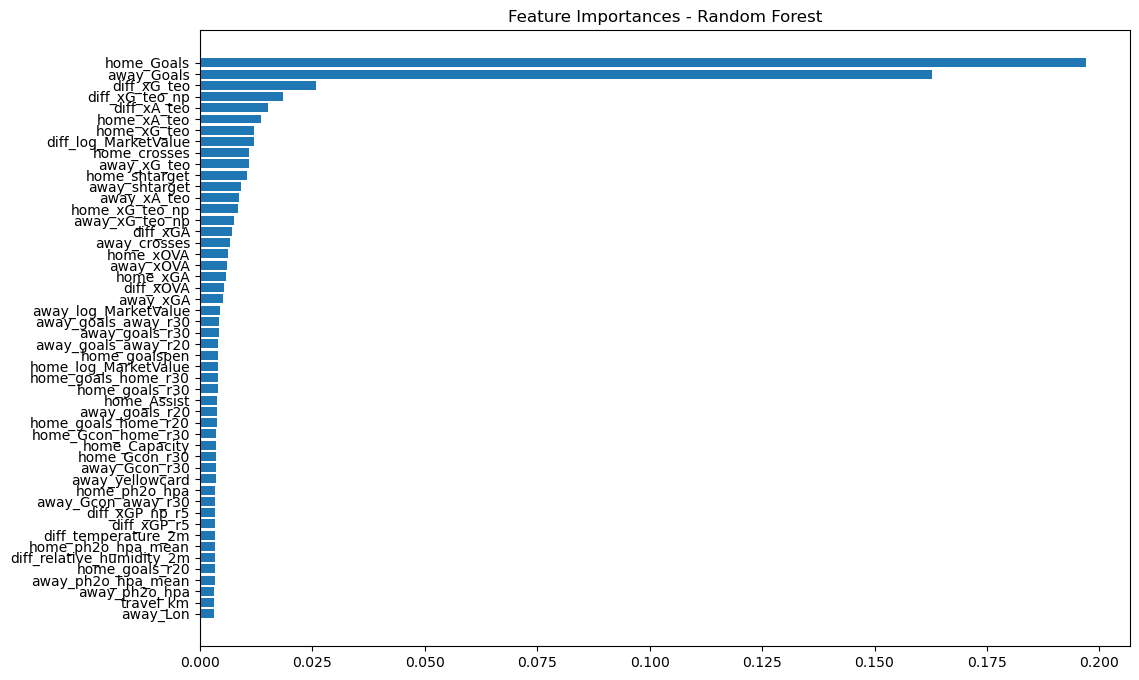
\includegraphics[width=0.9\textwidth]{primerforest.png}
	\caption{Distribuci\'on de la importancia de las caracter\'isticas en el primer clasificador Random Forest. Las dos variables dominantes son los goles del local y del visitante, lo que evidencia fuga de informaci\'on.}
	\label{fig:PrimerRandomForest}
\end{figure}

Asimismo, las variables macroecon\'omicas (PIB, inflaci\'on, Gini, gasto p\'ublico, deuda e IED) y sus transformaciones logar\'itmicas ocuparon posiciones marginales en el ranking de importancia, con valores inferiores a $0{.}004$ en todos los casos. Esto confirma su escasa se\~nal predictiva en la escala del resultado individual, en contraste con su relevancia documentada a nivel de temporada completa.

Con base en este diagn\'ostico se decidi\'o eliminar todas las variables derivadas directamente de los marcadores finales (\texttt{home\_Goals}, \texttt{away\_Goals} y sus promedios m\'oviles asociados); descartar el bloque macroecon\'omico del conjunto de caracter\'isticas activas, conserv\'andolo en el conjunto de datos maestro por reproducibilidad pero excluy\'endolo del modelo predictivo; y excluir las variables intermedias que presentaran redundancia con los \'indices compuestos de autor\'ia o que compartieran la misma fuente de fuga que los goles.

\paragraph{Segundo diagn\'ostico: filtrado y an\'alisis de importancias.} Sobre las decisiones anteriores se obtuvo un conjunto de datos filtrado que excluye las variables de fuga y conserva \'unicamente m\'etricas ex\'ogenas genuinamente disponibles antes del partido, m\'as las m\'etricas \textit{rolling} hist\'oricas. El mismo clasificador Random Forest se reentren\'o sobre este conjunto, con id\'entica partici\'on temporal.

El desempe\~no cay\'o dr\'asticamente a una \emph{accuracy} de $0{.}4879$ y un $F1$-score macro de $0{.}37$ sobre el conjunto de prueba, con las m\'etricas por clase recogidas en la parte derecha de la Tabla~\ref{tab:rf_diagnostico}.


La ca\'ida de m\'as de cuarenta puntos porcentuales en \emph{accuracy} al eliminar las variables de fuga confirma que la predicci\'on de resultados de f\'utbol es un problema de alta entrop\'ia cuando se restringe a informaci\'on disponible antes del partido. La matriz de confusi\'on (Figura~\ref{fig:SegundaMatrizConfusion}) revel\'o el patr\'on caracter\'istico ya discutido en el Marco Te\'orico: la clase empate colapsa casi por completo bajo una regla de decisi\'on dura $\arg\max$, con un \emph{recall} de apenas $0{.}03$, mientras que el modelo confunde sistem\'aticamente victorias locales y visitantes.

\begin{figure}[htbp]
	\centering
	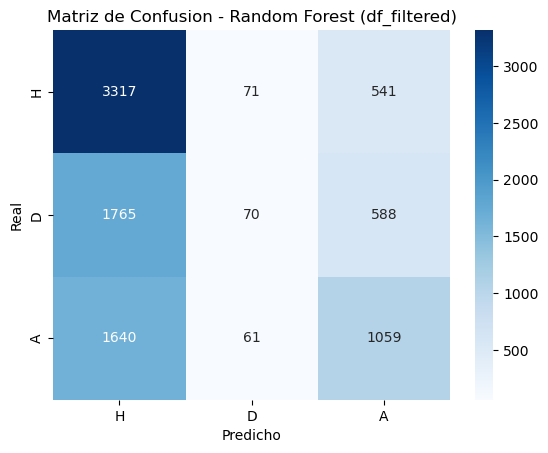
\includegraphics[width=0.9\textwidth]{matrizconfusion2.png}
	\caption{Matriz de confusi\'on del clasificador Random Forest sobre el conjunto filtrado. La clase empate colapsa bajo la regla $\arg\max$, en l\'inea con la dificultad estructural documentada en la Secci\'on~\ref{subsec:clasificacion}.}
	\label{fig:SegundaMatrizConfusion}
\end{figure}

El an\'alisis de importancias de Gini del modelo filtrado (Figura~\ref{fig:SegundoRandomForest}) permite identificar las variables con mayor peso relativo. Las seis covariables de mayor importancia fueron:
\begin{itemize}
	\item \texttt{diff\_MarketValue} ($0{.}0745$).
	\item \texttt{home\_Assist} ($0{.}0253$).
	\item \texttt{diff\_TDA} ($0{.}0224$).
	\item \texttt{diff\_xGP\_r5} ($0{.}0194$).
	\item \texttt{diff\_DDI} ($0{.}0190$).
	\item \texttt{travel\_km} ($0{.}0189$).
\end{itemize}
El resto de las variables present\'o importancias entre $0{.}010$ y $0{.}019$, sin una jerarqu\'ia pronunciada. Esta distribuci\'on, mucho m\'as plana que la del primer modelo, refleja que una vez eliminada la fuga de informaci\'on el problema se vuelve 
genuinamente dif\'icil y la se\~nal predictiva se distribuye entre m\'ultiples covariables. La variable \texttt{diff\_TDA} es un componente del \'indice de eficiencia defensiva \texttt{diff\_DDI}; su presencia individual en el ranking no implica que deba retenerse por separado, pues su informaci\'on ya est\'a capturada por el \'indice compuesto. El an\'alisis de selecci\'on multivariante de la subsecci\'on siguiente resuelve esta redundancia.

\begin{figure}[htbp]
	\centering
	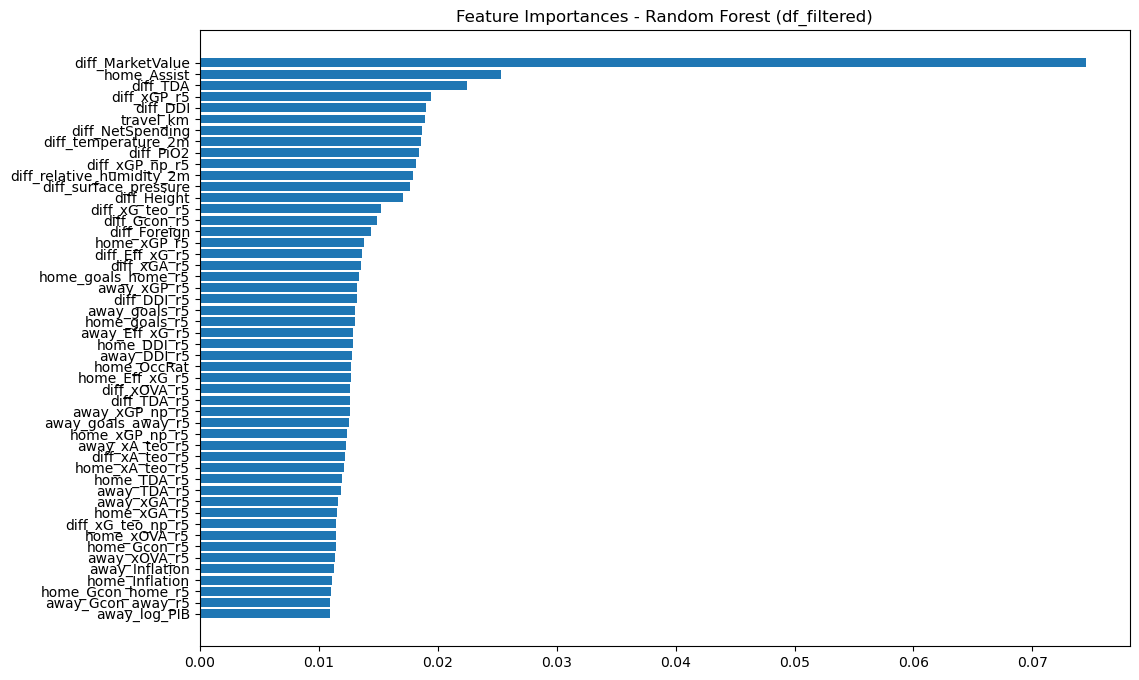
\includegraphics[width=0.9\textwidth]{segundoforest.png}
	\caption{Distribuci\'on de la importancia de las caracter\'isticas en el segundo clasificador Random Forest, tras eliminar las variables con fuga de informaci\'on.}
	\label{fig:SegundoRandomForest}
\end{figure}

En conjunto, los dos diagn\'osticos por Random Forest reducen el universo de aproximadamente 192 variables derivadas a un conjunto acotado de covariables candidatas, descartando las fuentes de fuga y las redundancias estructurales. Sobre ese conjunto acotado se aplican a continuaci\'on tres criterios de selecci\'on complementarios, con el objetivo de construir un ranking consolidado y fijar el vector de entrada del modelo de refinamiento.

\subsection{Criterios de selecci\'on multivariante}
\label{subsec:criterios_seleccion}

Sobre el subconjunto de covariables candidatas resultante del diagn\'ostico anterior se aplicaron tres criterios complementarios de selecci\'on, con el objetivo de combinar informaci\'on de distinta naturaleza estad\'istica y de depurar la redundancia residual entre variables afines. A diferencia de los clasificadores Random Forest empleados en las dos diagn\'osticos previos, cuyo universo de variables derivadas era m\'as amplio y a\'un reten\'ia variables redundantes, los tres criterios de esta subsecci\'on operan exclusivamente sobre el conjunto final de covariables candidatas. En consecuencia, las importancias relativas que se reportan a continuaci\'on no son directamente comparables con las de la Secci\'on~\ref{subsec:segunda_pasada}. Los tres criterios son: la correlaci\'on de Spearman \cite{spearman1904} de cada variable con el resultado codificado ordinalmente (victoria local $=2$, empate $=1$, victoria visitante $=0$), tomada en valor absoluto; la importancia de Gini de un clasificador Random Forest reentrenado sobre el mismo conjunto, que captura asociaciones no lineales y de orden superior; y el coeficiente promedio de una regresi\'on log\'istica con penalizaci\'on $L_1$, que induce esparsidad al anular los coeficientes de variables redundantes. Las covariables se estandarizaron previamente para el tercer criterio, ya que la penalizaci\'on $L_1$ opera sobre magnitudes.

Cada criterio se normaliz\'o al intervalo $[0,1]$ mediante escalamiento MinMax y los tres valores normalizados se sumaron para producir un \emph{score} consolidado por variable. Este score alcanza su valor m\'aximo posible de $3{.}000$ cuando una variable ocupa la primera posici\'on en los tres criterios simult\'aneamente. La Tabla~\ref{tab:ranking_variables} presenta el ranking consolidado para los conjuntos de datos Lite y Full.

\begin{table}[htbp]
	\centering
	\caption{Ranking consolidado de importancia de variables para los conjuntos de datos Lite y Full. Las columnas ``Sp.'', ``RF'' y ``L1'' corresponden a la correlaci\'on de Spearman (valor absoluto), la importancia en Random Forest y el coeficiente $L_1$ promedio (absoluto entre clases), respectivamente. El score total es la suma de los tres criterios normalizados con MinMax, con m\'aximo posible de $3{.}000$.}
	\label{tab:ranking_variables}
	\small
	\begin{tabular}{lcccc|lcccc}
		\toprule
		& \multicolumn{4}{c}{\textbf{Dataset Lite}} & & 
		\multicolumn{4}{c}{\textbf{Dataset Full}} \\
		\cmidrule(lr){2-5} \cmidrule(lr){7-10}
		\textbf{Variable} & \textbf{Sp.} & \textbf{RF} & 
		\textbf{L1} & \textbf{Total} & & \textbf{Sp.} & 
		\textbf{RF} & \textbf{L1} & \textbf{Total} \\
		\midrule
		diff\_MarketValue & 0.274 & 0.170 & 0.205 & 3.000 & & 0.276 & 0.134 & 0.194 & 3.000 \\
		diff\_xG\_teo\_r5 & ---   & ---   & ---   & ---   & & 0.158 & 0.082 & 0.077 & 1.218 \\
		home\_Assist & 0.108 & 0.114 & 0.060 & 1.018 & & 0.112 & 0.088 & 0.058 & 1.033 \\
		travel\_km & 0.034 & 0.134 & 0.022 & 0.783 & & 0.037 & 0.098 & 0.024 & 0.724 \\
		diff\_NetSpending & 0.053 & 0.117 & 0.002 & 0.570 & & 0.052 & 0.091 & 0.009 & 0.604 \\
		diff\_PiO2 & 0.006 & 0.141 & 0.015 & 0.731 & & 0.012 & 0.101 & 0.002 & 0.568 \\
		diff\_xA\_teo\_r5 & --- & --- & ---   & --- & & 0.041 & 0.081 & 0.028 & 0.519 \\
		home\_OccRat & 0.047 & 0.109 & 0.003 & 0.459 & & 0.047 & 0.083 & 0.005 & 0.447 \\
		diff\_temperature\_2m & 0.013 & 0.131 & 0.002 & 0.580 & & 0.001 & 0.095 & 0.002 & 0.436 \\
		diff\_DDI\_r5 & --- & --- & --- & ---  & & 0.017 & 0.081 & 0.010 & 0.327 \\
		diff\_Foreign & 0.055 & 0.083 & 0.002 & 0.181 & & 0.043 & 0.065 & 0.008 & 0.185 \\
		\bottomrule
	\end{tabular}
\end{table}

\subsection{An\'alisis de ablaci\'on y conjunto final de covariables}
\label{subsec:conjunto_final}

Para cuantificar el aporte marginal de las covariables candidatas, se realiz\'o un an\'alisis de ablaci\'on \emph{leave-one-out} mediante validaci\'on cruzada con 10 particiones aleatorias (\emph{shuffle}), utilizando el mismo clasificador Random Forest y comparando los resultados con pruebas $t$ pareadas. Es importante destacar que este an\'alisis tiene prop\'osito de diagn\'ostico, no de reporte del rendimiento final del sistema; las m\'etricas aqu\'i obtenidas no son directamente comparables con las del \textit{pipeline} principal, que utiliza una partici\'on cronol\'ogica estricta.

\paragraph{Resultados sobre los conjuntos de datos Lite y Full.} Los 
resultados de la ablaci\'on se resumen en la 
Tabla~\ref{tab:ablacion}. Ninguna de las diferencias entre configuraciones alcanza significancia al $5\%$, ni en \emph{accuracy} ni en $F1$-macro, en ninguno de los dos conjuntos de datos.

\begin{table}[htbp]
	\centering
	\caption{An\'alisis de ablaci\'on por validaci\'on cruzada con 
		10 particiones. Media $\pm$ desviaci\'on est\'andar y 
		$p$-valor del test $t$ pareado contra la configuraci\'on 
		completa.}
	\label{tab:ablacion}
	\small
	\begin{tabular}{llcccc}
		\toprule
		& & \multicolumn{2}{c}{\textbf{Dataset Lite}} & 
		\multicolumn{2}{c}{\textbf{Dataset Full}} \\
		\cmidrule(lr){3-4} \cmidrule(lr){5-6}
		\textbf{M\'etrica} & \textbf{Configuraci\'on} & 
		Valor & $p$ & Valor & $p$ \\
		\midrule
		\multirow{3}{*}{Accuracy}
		& Todas las variables          & $0.4550 \pm 0.0066$ & ---     & $0.4638 \pm 0.0103$ & --- \\
		& Sin \texttt{home\_OccRat}    & $0.4562 \pm 0.0060$ & 0.4564  & $0.4626 \pm 0.0075$ & 0.6805 \\
		& Sin \texttt{travel\_km}      & $0.4571 \pm 0.0053$ & 0.3780  & $0.4636 \pm 0.0087$ & 0.9505 \\
		\midrule
		\multirow{3}{*}{$F1$-macro}
		& Todas las variables          & $0.3955 \pm 0.0084$ & ---     & $0.3921 \pm 0.0078$ & --- \\
		& Sin \texttt{home\_OccRat}    & $0.3965 \pm 0.0055$ & 0.6177  & $0.3904 \pm 0.0085$ & 0.5364 \\
		& Sin \texttt{travel\_km}      & $0.4005 \pm 0.0049$ & 0.0817  & $0.3936 \pm 0.0077$ & 0.5784 \\
		\bottomrule
	\end{tabular}
\end{table}

Los resultados anteriores muestran que ninguna de las covariables candidatas aporta una mejora estad\'isticamente significativa al modelo por s\'i sola: todas las diferencias entre configuraciones son compatibles con la hip\'otesis nula de aporte nulo. La decisi\'on de retenci\'on se apoy\'o entonces en dos criterios complementarios: la existencia de redundancia estructural entre variables afines, y la posici\'on relativa de cada covariable en el ranking consolidado de la Tabla~\ref{tab:ranking_variables}. Los dos casos que requieren discusi\'on expl\'icita son \texttt{home\_OccRat} y \texttt{travel\_km}.

\paragraph{Decisi\'on sobre \texttt{home\_OccRat}.} La variable 
\texttt{home\_OccRat} es una transformaci\'on determinista de \texttt{home\_Assist} (Ecuaci\'on~\ref{eq:OccRat}), lo que genera una redundancia estructural entre ambas. El ranking consolidado muestra que \texttt{home\_Assist} supera consistentemente a \texttt{home\_OccRat} en los tres criterios considerados: $1{.}018$ vs $0{.}459$ en el Dataset Lite y $1{.}033$ vs $0{.}447$ en el Dataset Full. El an\'alisis de ablaci\'on confirma que la exclusi\'on de \texttt{home\_OccRat} no degrada el rendimiento ($p > 0.45$ en ambos conjuntos de datos). En consecuencia, se descarta \texttt{home\_OccRat} y se retiene \texttt{home\_Assist} como representante del bloque de estadio y afici\'on. La Tabla~\ref{tab:correlacion_spearman} reporta la matriz de correlaci\'on de rangos entre las covariables del bloque ex\'ogeno, que respalda esta decisi\'on desde el \'angulo de los coeficientes de Spearman.

\begin{table}[htbp]
	\centering
	\caption{Coeficientes de correlaci\'on de Spearman entre las covariables del bloque ex\'ogeno, para los pares con $|\rho| > 0{.}10$. La matriz se calcul\'o sobre las covariables disponibles al momento del an\'alisis de selecci\'on; no incluye \texttt{diff\_NetSpending} ni \texttt{travel\_km}, incorporadas al conjunto final con posterioridad.}
	\label{tab:correlacion_spearman}
	\begin{tabular}{lcc}
		\toprule
		\textbf{Par de variables} & \textbf{Lite} & \textbf{Full} \\
		\midrule
		\texttt{home\_Assist}--\texttt{home\_OccRat} & $0{.}784$ & $0{.}753$ \\
		\texttt{diff\_MarketValue}--\texttt{diff\_xG\_teo\_r5} & --- & $0{.}310$ \\
		\texttt{diff\_MarketValue}--\texttt{diff\_Foreign} & $0{.}225$ & $0{.}220$ \\
		\texttt{diff\_MarketValue}--\texttt{home\_Assist} & $0{.}216$ & $0{.}224$ \\
		\texttt{diff\_temperature\_2m}--\texttt{diff\_PiO2} & $0{.}194$ & $0{.}101$ \\
		\texttt{diff\_xG\_teo\_r5}--\texttt{diff\_xA\_teo\_r5} & --- & $0{.}119$ \\
		\bottomrule
	\end{tabular}
\end{table}

El \'unico par de covariables que supera el umbral de $0{.}5$ es \texttt{home\_Assist}--\texttt{home\_OccRat}, con $0{.}784$ en Lite y $0{.}753$ en Full, lo que confirma cuantitativamente la redundancia estructural entre ambas. Los pares restantes se mantienen por debajo de $0{.}35$, y la mayor\'ia por debajo de $0{.}25$. Los tres pares que involucran a \texttt{diff\_MarketValue} con \texttt{diff\_xG\_teo\_r5}, \texttt{diff\_Foreign} y \texttt{home\_Assist} presentan coeficientes en torno a $0{.}22$ y son consistentes con la interpretaci\'on de que el valor de mercado funciona como un indicador agregado de la calidad del club, que se refleja simult\'aneamente en la generaci\'on de ocasiones, la composici\'on de la plantilla y el respaldo de la afici\'on. La baja correlaci\'on entre \texttt{diff\_temperature\_2m} y \texttt{diff\_PiO2} confirma que, aunque ambas variables pertenecen al bloque ambiental, capturan efectos f\'isicos distintos. En conjunto, la matriz respalda la decisi\'on de descartar \texttt{home\_OccRat} y confirma que las covariables restantes son suficientemente independientes entre s\'i para alimentar el refinamiento no lineal sin inducir multicolinealidad.

\paragraph{Decisi\'on sobre \texttt{travel\_km}.} La variable \texttt{travel\_km} presenta un $p$-valor de $0{.}3780$ en el Dataset Lite y $0{.}9505$ en el Full, lo que indica que su eliminaci\'on no afecta significativamente la \emph{accuracy} en ning\'un caso. Su relevancia en el ranking consolidado es alta (posici\'on 3 en Lite con score $0{.}783$, posici\'on 4 en Full con $0{.}724$). En el Dataset Lite, su eliminaci\'on mejora marginalmente el $F1$-macro ($0{.}3955 \to 0{.}4005$, $p = 0{.}0817$) y la \emph{accuracy} ($0{.}4550 \to 0{.}4571$), sin alcanzar significancia al $5\%$; en el Dataset Full el efecto es nulo. Dado que la literatura base sobre ventaja de local\'ia se\~nala el desplazamiento geogr\'afico como un factor estructural \cite{Glicko2Mod}, y que su efecto sobre el desempe\~no es despreciable en ambos conjuntos de datos, se decide mantener \texttt{travel\_km} en el conjunto final.

\paragraph{Conjunto final de covariables ex\'ogenas.} El conjunto activo que alimenta el perceptr\'on multicapa queda conformado por siete variables en el Dataset Lite y el Dataset Lite Recortado, y diez en el Dataset Full:

\begin{itemize}
	\item \textbf{Bloque econ\'omico:} \texttt{diff\_MarketValue}, \texttt{diff\_NetSpending}.
	\item \textbf{Bloque de composici\'on de plantilla:} \texttt{diff\_Foreign}.
	\item \textbf{Bloque ambiental y geogr\'afico:} \texttt{diff\_temperature\_2m}, \texttt{diff\_PiO2}, \texttt{travel\_km}.
	\item \textbf{Bloque de estadio y afici\'on:} \texttt{home\_Assist}.
	\item \textbf{Bloque deportivo} (solo en el Dataset Full): \texttt{diff\_xG\_teo\_r5}, \texttt{diff\_xA\_teo\_r5}, \texttt{diff\_DDI\_r5}.
\end{itemize}

Este vector, junto con las tres probabilidades base $(P_H, P_D, P_A)$ generadas por el sistema de rating y el modelo de conteo, constituye el input $\mathbf{z}_{ij} \in \mathbb{R}^{d}$ del MLP, donde $d=10$ en el Dataset Lite y Lite Recortado, y $d=13$ en el Dataset Full. La reducci\'on dimensional busc\'o mitigar el sobreajuste en la fase de refinamiento no lineal, aunque el dr\'astico descenso de \emph{accuracy} entre el primer y segundo diagn\'ostico del Random Forest sugiere que el cuello de botella del sistema no reside en la dimensionalidad, sino en la alta varianza inherente al fen\'omeno deportivo. El an\'alisis detallado del desempe\~no predictivo del \textit{pipeline} completo se reserva para el Cap\'itulo~\ref{ch:resultados}.

% ============================================================
% SECCION 3.4 -- Arquitectura y calibracion del sistema predictivo
% ============================================================

\section{Arquitectura y calibraci\'on del sistema predictivo}
\label{sec:arquitectura}

El sistema predictivo se organiza como un \textit{pipeline} de tres bloques funcionales encadenados: un bloque de conteo que estima las tasas de goles y deriva una probabilidad de empate; un bloque de rating din\'amico que actualiza secuencialmente la fuerza latente de los equipos y genera un vector de probabilidades base; y un bloque de refinamiento no param\'etrico que corrige dichas probabilidades mediante un perceptr\'on multicapa alimentado con covariables ex\'ogenas. Esta secci\'on documenta las decisiones de dise\~no de cada bloque y el procedimiento de calibraci\'on utilizado, respetando estrictamente el orden de dependencias del sistema: el bloque de conteo se entrena primero, sus predicciones alimentan la calibraci\'on del rating, y las probabilidades base de este \'ultimo alimentan el entrenamiento del refinador neuronal. Los valores num\'ericos obtenidos en cada etapa de calibraci\'on y entrenamiento se reportan en el Cap\'itulo~\ref{ch:resultados}.

La variable a predecir en todos los bloques es el resultado del partido al finalizar el tiempo reglamentario, codificada en tres clases mutuamente excluyentes: victoria del equipo local ($H$), empate ($D$) o victoria del equipo visitante ($A$). La codificaci\'on operativa difiere entre bloques seg\'un la naturaleza de cada uno. En el bloque de rating se representa mediante el escalar $s_j \in \{1, 0{.}5, 0\}$ seg\'un el resultado observado, notaci\'on can\'onica de los sistemas Elo y Glicko. Para el bloque de refinamiento (MLP), la codificaci\'on se transforma a un vector indicador \emph{one-hot} $\mathbf{y}_i \in \{0,1\}^3$, donde la componente correspondiente a la clase observada toma valor $1$ y las restantes $0$.

\subsection{Bloque de conteo: estimaci\'on de tasas y probabilidad de empate}
\label{subsec:conteo}

El primer bloque modela el n\'umero de goles anotados por cada equipo como un proceso de conteo independiente, siguiendo el marco te\'orico de la Secci\'on~\ref{sec:modelo_probabilistico}. Se entrenan dos regresores LightGBM con funci\'on objetivo Poisson \cite{ke2017lightgbm}, uno para los goles del equipo local ($\lambda_H$) y otro para los del visitante ($\lambda_A$).

\paragraph{Partici\'on temporal.} La partici\'on respeta el orden cronol\'ogico: el $70\%$ inicial de los partidos (ordenados por \texttt{match\_date\_from\_id}) constituye el conjunto de entrenamiento; el $30\%$ restante, el de prueba. Dentro del entrenamiento se reserva un $10\%$ final para \emph{early stopping}. Este dise\~no evita la fuga de informaci\'on temporal y garantiza que el modelo solo utiliza partidos anteriores a los de prueba.

\paragraph{Variables de entrada.} Dado que el objetivo de este bloque es capturar la din\'amica de forma reciente sin introducir fuga del resultado final, \'unicamente se utilizan las variables de promedios m\'oviles de goles anotados y recibidos en ventanas de $5$, $10$, $20$ y $30$ partidos, diferenciadas por condici\'on de local\'ia. Espec\'ificamente, las entradas son $32$ columnas que cruzan cuatro dimensiones:
\begin{enumerate}
	\item El prefijo indica si la estad\'istica corresponde al equipo 	local (\texttt{home}) o al visitante (\texttt{away}).
	\item La ra\'iz distingue entre goles marcados (\texttt{goals}) y goles recibidos (\texttt{Gcon}).
	\item Para cada prefijo se generan dos versiones: la global, sin sufijo adicional, y la condicionada a partidos jugados en la condici\'on del prefijo.
	\item El sufijo final determina el tama\~no de la ventana, que puede ser $5$, $10$, $20$ o $30$ partidos.
\end{enumerate}
El producto de estas dimensiones, $2 \times 2 \times 2 \times 4 = 32$, da como resultado las $32$ columnas del grupo.

\paragraph{Hiperpar\'ametros.} Los modelos se configuran con \texttt{n\_estimators}$=200$, \texttt{learning\_rate}$=0{.}05$, \texttt{max\_depth}$=5$ y criterio de parada temprana de $10$ iteraciones sin mejora en el MAE de validaci\'on. La m\'etrica de evaluaci\'on interna es el error absoluto medio, coherente con la escala de conteo de los goles.

\paragraph{Derivaci\'on de la probabilidad de empate.} A partir de las tasas predichas $\hat{\lambda}_H$ y $\hat{\lambda}_A$, se calcula la probabilidad de empate mediante la distribuci\'on de Skellam evaluada en $k=0$ (Ecuaci\'on~\ref{eq:prob_D_bessel} del Cap\'itulo~\ref{ch:marco}):
\begin{equation}
	\hat{P}_D^{(S)} = e^{-(\hat{\lambda}_H + \hat{\lambda}_A)} \, 
	I_0\!\left(2\sqrt{\hat{\lambda}_H \hat{\lambda}_A}\right).
\end{equation}
Este valor, denominado \texttt{draw\_prob} en el \textit{pipeline}, se anexa al conjunto de datos y alimenta el bloque de rating como estimaci\'on externa de la frecuencia de empates.

\subsection{Bloque de rating: Glicko-2 modificado}
\label{subsec:rating}

El n\'ucleo inferencial del sistema es una implementaci\'on propia basada en el algoritmo Glicko-2 modificado de Shelopugin y Sirotkin \cite{Glicko2Mod}, contenida en el m\'odulo \texttt{G2Av1513.py}. A diferencia del motor can\'onico de referencia (\texttt{glicko2.py}), esta implementaci\'on incorpora varias mejoras de mecanismos num\'ericos y coherencia probabil\'istica que se detallan a continuaci\'on.

\subsubsection{Diferencias frente al motor de referencia}
\label{subsubsec:mejoras_g2av1513}

El motor \texttt{G2Av1513.py} se construy\'o sobre el c\'odigo can\'onico de Shelopugin y Sirotkin (\texttt{glicko2.py}), del cual hereda la estructura de actualizaci\'on bayesiana del Glicko-2. Sobre esa base se introdujeron tres clases de modificaciones, que se distinguen por su naturaleza: correcciones algebraicas que alteran el comportamiento probabil\'istico del modelo, decisiones de calibraci\'on emp\'irica respaldadas por barridos de hiperpar\'ametros, y mecanismos de estabilidad num\'erica que preservan el comportamiento del motor en condiciones extremas sin alterar sus predicciones en r\'egimen normal. Se documentan tambi\'en dos extensiones funcionales que quedaron implementadas pero no activadas en el \textit{pipeline} principal.

\paragraph{Correcci\'on del denominador trinomial.} El motor de referencia computa las tres probabilidades mediante dos denominadores asim\'etricos respecto al t\'ermino de empate. La probabilidad de victoria local surge del denominador $1 + (1 + e^{d+P_D^{(S)}})/e^{\delta}$ y la de victoria visitante de $1 + (1 + e^{d+P_D^{(S)}})e^{\delta}$, donde $\delta = g(\phi_j)(\mu - \mu_j)$ es la diferencia de ratings efectiva y $P_D^{(S)}$ la probabilidad de empate derivada de la distribuci\'on de Skellam. La probabilidad de empate se obtiene por complemento, $P_D = 1 - P_H - P_A$. Esta construcci\'on asigna al par\'ametro $d$ un efecto que depende de $\delta$ en lugar de operar como t\'ermino sim\'etrico del empate: a medida que la diferencia de ratings crece, el denominador de la victoria visitante crece con $\delta$ y el de la victoria local decrece, de modo que el empate queda estructuralmente penalizado en partidos desequilibrados. El motor propio unifica el denominador como
\begin{equation}
	1 + \exp(\delta) + \exp(d + P_{D,\text{logit}}^{(S)}),
\end{equation}
garantizando que las tres probabilidades provengan de una partici\'on sim\'etrica del simplex y que $d$ act\'ue como un t\'ermino aditivo puro sobre la masa del empate.

\paragraph{Reparametrizaci\'on logit del par\'ametro de empate.} El motor can\'onico alimenta la probabilidad de empate cruda $P_D^{(S)} \in (0,1)$ directamente al exponente $\exp(d+P_D^{(S)})$. Como $P_D^{(S)}$ var\'ia aproximadamente en $[0.2, 0.3]$ en el rango operativo del f\'utbol profesional, el t\'ermino $\exp(d+P_D^{(S)})$ es pr\'acticamente constante y el par\'ametro de empate resulta funcionalmente inerte frente a la se\~nal del modelo de conteo. La implementaci\'on propia aplica la transformaci\'on logit
\begin{equation}
	P_{D,\text{logit}}^{(S)} = \ln\!\left(\frac{P_{D}^{(S)}}{1-P_{D}^{(S)}}\right),
\end{equation}
que mapea $(0,1)$ sobre la recta real y preserva la variabilidad de la se\~nal de Skellam dentro del exponente. Esta correcci\'on es funcional, no un simple cambio de escala, pues altera la forma en que el modelo responde a variaciones en la probabilidad de empate del bloque de conteo.

\paragraph{Calibraci\'on emp\'irica de la constante de atenuaci\'on y la volatilidad.} Dos hiperpar\'ametros heredados del motor can\'onico fueron reajustados mediante un barrido emp\'irico sobre el panel multiliga. La constante de atenuaci\'on $g$ del factor $g(\phi_j)$ pas\'o de $1{.}5/\pi^2$ a $3{.}0/\pi^2$, lo que suaviza la superficie de p\'erdida del optimizador y reduce la sensibilidad del rating a la diferencia de desviaciones entre equipos. La constante de difusi\'on temporal $\tau$ pas\'o de $1{.}0$ a $0{.}8$, valor que produce una trayectoria de volatilidad m\'as estable sobre el panel utilizado. Ambos ajustes se derivaron de un barrido de configuraciones previo a la arquitectura en cascada final y se fijaron por su desempe\~no en la log-loss de validaci\'on del bloque de rating en aislamiento.

\paragraph{Mecanismos de estabilidad num\'erica.} La calibraci\'on por L-BFGS-B sobre un panel multiliga expone al motor a reg\'imenes num\'ericos extremos que el c\'odigo can\'onico no contempla. Se a\~nadieron acotamientos sobre la diferencia de ratings efectiva, sobre la puntuaci\'on esperada antes del c\'alculo de la varianza $v$, sobre las probabilidades finales del simplex, y una protecci\'on contra divisi\'on por cero en la funci\'on de varianza. Estos mecanismos no alteran el comportamiento del motor en r\'egimen normal; su funci\'on es evitar indeterminaciones num\'ericas cuando el optimizador explora regiones alejadas del \'optimo durante la calibraci\'on.

\paragraph{Extensiones funcionales no activadas.} El motor propio incorpora dos extensiones que no se utilizan en el \textit{pipeline} del presente trabajo pero quedan disponibles para desarrollos futuros. La primera es un sistema de ventaja parametrizada: mientras el motor can\'onico recibe un escalar fijo \texttt{advantage}, el motor propio acepta un vector de covariables y calcula la ventaja efectiva como combinaci\'on lineal $h_{\text{eff}} = \beta_0 + \sum_k \beta_k f_k$. En la versi\'on calibrada esta flexibilidad se emplea \'unicamente para inyectar la ventaja de local\'ia por liga $h_\ell$ como \'unico para\'ametro activo, dejando la infraestructura disponible para extensiones. La segunda corresponde a una atenuaci\'on multiplicativa de la ventaja de local\'ia, definida originalmente para ser utilizada durante el per\'iodo marzo 2020--junio 2021, durante la pandemia global de la COVID-19, esta funci\'on se encuentra descrita en el trabajo base pero no implementada en su c\'odigo. En esta implementaci\'on la extensi\'on est\'a codificada y se activa con un indicador binario; en todas las ejecuciones del presente trabajo dicho indicador toma valor $0$.

La Tabla~\ref{tab:constantes_divergentes} consolida los hiperpar\'ametros donde la implementaci\'on propia se aparta del valor can\'onico de Glicko-2 o del motor de referencia de Shelopugin y Sirotkin. Los tres valores se fijaron emp\'iricamente mediante un barrido de configuraciones previo a la arquitectura en cascada final; no provienen de una regla derivada de la literatura, sino de su desempe\~no en la log-loss de validaci\'on del bloque de rating en aislamiento.

\begin{table}[htbp]
	\centering
	\caption{Hiperpar\'ametros donde la implementaci\'on se aparta del valor can\'onico.}
	\label{tab:constantes_divergentes}
	\small
	\begin{tabular}{p{2.8cm} p{2.6cm} p{2.6cm} p{6.4cm}}
		\toprule
		\textbf{Par\'ametro} & \textbf{Valor can\'onico} & \textbf{Valor implementado} & \textbf{Justificaci\'on} \\
		\midrule
		$RD_0$ & $350$ & $80$ & La calibraci\'on preliminar mostr\'o una convergencia m\'as estable del optimizador sobre el panel multiliga. \\
		$\tau$ & $1{.}0$ & $0{.}8$ & El barrido emp\'irico produjo una trayectoria de volatilidad m\'as estable sobre el panel utilizado. \\
		$g_{\text{constant}}$ & $1{.}5/\pi^2$ & $3{.}0/\pi^2$ & Suaviza la superficie de p\'erdida del optimizador y reduce la sensibilidad del rating a la diferencia de desviaciones entre equipos. \\
		\bottomrule
	\end{tabular}
\end{table}

\begin{obs}[Sobre la funci\'on de actualizaci\'on de volatilidad]
	Tanto el motor can\'onico de Shelopugin y Sirotkin como la implementaci\'on propia omiten el factor $\tau^2$ en el denominador del segundo t\'ermino de la funci\'on $f(x)$ del Paso~5 del algoritmo Glicko-2. Esta simplificaci\'on, heredada del c\'odigo fuente de referencia, no impide la convergencia del m\'etodo de Illinois empleado para la estimaci\'on de $\sigma'$, aunque desv\'ia ligeramente la trayectoria de optimizaci\'on respecto a la formulaci\'on can\'onica de Glickman \cite{Glickman2022}. Dado que ambos motores comparten esta misma estructura, no se documenta como diferencia del presente trabajo.
\end{obs}

\subsubsection{Calibraci\'on por m\'axima verosimilitud}
\label{subsubsec:calibracion_glicko}

El bloque de rating se calibra sobre cada conjunto de datos por separado mediante la minimizaci\'on de la log-verosimilitud negativa del resultado observado. Formalmente, sea $\mathcal{D}_{\text{train}}$ el conjunto de partidos ordenados cronol\'ogicamente. Para cada partido $i$, el modelo genera el vector $(P_{H,i}, P_{D,i}, P_{A,i})$ seg\'un las Ecuaciones~\eqref{eq:prob_victoria_local}--\eqref{eq:prob_victoria_visitante} del Cap\'itulo~\ref{ch:marco}, y actualiza secuencialmente los ratings de ambos equipos. La funci\'on objetivo es
\begin{equation}
	\mathcal{L}_{\text{G2A}}(d, \{\mu_{\text{init},\ell}\}, \{h_\ell\}) 
	= -\frac{1}{|\mathcal{D}_{\text{train}}|}
	\sum_{i \in \mathcal{D}_{\text{train}}} \log P_{o_i,i},
\end{equation}
donde $o_i \in \{H,D,A\}$ es el resultado observado y $P_{o_i,i}$ la probabilidad asignada a dicha clase.

\paragraph{Espacio de par\'ametros y cotas.} El optimizador L-BFGS-B \cite{byrd1995limited} ajusta simult\'aneamente los hiperpar\'ametros estructurales del bloque, restringidos a intervalos derivados de su interpretaci\'on probabil\'istica:
\begin{itemize}
	\item El t\'ermino de calibraci\'on del empate $d \in [-5{.}0,\, 5{.}0]$.
	\item El rating inicial medio por liga 	$\mu_{\text{init},\ell} \in [1200,\, 1800]$, expresado como desviaci\'on respecto a $1500$ en el espacio de optimizaci\'on.
	\item La ventaja de local\'ia por liga $h_\ell \in [0,\, 200]$, escalada internamente por un factor $10$ en el optimizador.
\end{itemize}
Los valores semilla son $d_0 = 0{.}5$, desviaciones nulas para $\mu_{\text{init},\ell}$ y valor escalado $5{.}0$ para $h_\ell$. El n\'umero m\'aximo de iteraciones del optimizador es $400$ y el criterio de convergencia es \texttt{ftol}$=10^{-5}$. La cota del t\'ermino de empate $d$ acota la correcci\'on sobre la probabilidad derivada de Skellam dentro de un rango de sensibilidad razonable; las cotas de $\mu_{\text{init},\ell}$ restringen el rating inicial a un entorno de 300 puntos alrededor del valor can\'onico 1500; y las cotas de $h_\ell$ corresponden a un efecto m\'aximo de 200 puntos de rating, equivalente a una ventaja de local\'ia fuerte pero no arbitraria.

\paragraph{Estado e inicializaci\'on.} Cada equipo se caracteriza por el estado $(R, RD, \sigma)$. Los valores iniciales por defecto son $R_0 = 1500$, $RD_0 = 80$ y $\sigma_0 = 0{.}06$. La constante de difusi\'on temporal se fija en $\tau = 0{.}8$, valor est\'andar para conjuntos de resultados de alta volatilidad \cite{Glickman2022}. Aunque el valor can\'onico de Glickman es $RD_0=350$, en esta implementaci\'on se fija $RD_0=80$ tras una calibraci\'on preliminar que mostr\'o una convergencia m\'as estable para el panel de ligas utilizado.

Los valores calibrados de $d$, $\mu_{\text{init},\ell}$ y $h_\ell$ por liga, as\'i como las estad\'isticas de convergencia del optimizador y el rango final de ratings, se reportan en la Secci\'on~\ref{sec:res_rating} del Cap\'itulo~\ref{ch:resultados}.

\subsection{Bloque de refinamiento: perceptr\'on multicapa}
\label{subsec:mlp}

El tercer bloque corrige las probabilidades base del Glicko-2 mediante un perceptr\'on multicapa \emph{feedforward} implementado en \texttt{Keras/TensorFlow}. La elecci\'on responde al car\'acter no lineal ni aditivo de las interacciones entre covariables y resultado: los tres criterios de selecci\'on de la Secci\'on~\ref{sec:seleccion_covariables} identificaron variables con se\~nal marginal, cuya contribuci\'on conjunta solo puede capturarse mediante una funci\'on de aproximaci\'on flexible. El Teorema de Aproximaci\'on Universal (Secci\'on~\ref{sec:mlp} del Cap\'itulo~\ref{ch:marco}) garantiza que una red con una capa oculta puede aproximar cualquier funci\'on continua sobre un compacto, propiedad que sostiene el uso del MLP como refinador no param\'etrico.

\paragraph{Vector de entrada.} La entrada del MLP combina las probabilidades base del rating con las covariables ex\'ogenas seleccionadas en las Secci\'on~\ref{sec:seleccion_covariables}. Para cada partido $i$, el vector $\mathbf{z}_{ij} \in \mathbb{R}^{d}$ se construye concatenando:
\begin{itemize}
	\item Las tres probabilidades base del Glicko-2: $(P_{H,i}, P_{D,i}, P_{A,i})$.
	\item Las covariables ex\'ogenas estandarizadas seleccionadas en la Secci\'on~\ref{sec:seleccion_covariables}: siete variables en los conjuntos de datos Lite y Lite Recortado (\texttt{diff\_MarketValue}, \texttt{diff\_NetSpending}, \texttt{diff\_Foreign}, \texttt{diff\_temperature\_2m}, \texttt{diff\_PiO2}, \texttt{travel\_km}, \texttt{home\_Assist}); y esas mismas siete m\'as las tres m\'etricas deportivas \textit{rolling} (\texttt{diff\_xG\_teo\_r5}, \texttt{diff\_xA\_teo\_r5}, \texttt{diff\_DDI\_r5}) en el Dataset Full.
\end{itemize}
En consecuencia, $d = 10$ para el Dataset Lite y el Dataset Lite Recortado, y $d = 13$ para el Dataset Full. La estandarizaci\'on de media cero y varianza unitaria se ajusta exclusivamente sobre el conjunto de entrenamiento mediante \texttt{StandardScaler} de \texttt{scikit-learn} y se aplica al conjunto de prueba.

\paragraph{Arquitectura e hiperpar\'ametros.} La red se estructura con dos capas ocultas densas de 64 neuronas cada una, precediendo una capa de salida con activaci\'on \emph{softmax} que garantiza un vector de probabilidades sobre las tres clases. La elecci\'on de ReLU en las capas ocultas y softmax en la salida sigue las recomendaciones est\'andar para clasificaci\'on multiclase \cite{solorzano2025rn}.

La profundidad de dos capas ocultas se fija por parsimonia: suficiente para capturar interacciones de segundo orden entre covariables, sin incurrir en la complejidad de una red profunda que el tama\~no del panel no justifica. La topolog\'ia resultante es:
\begin{itemize}
	\item Capa de entrada: $d$ neuronas, sin activaci\'on.
	\item Primera capa oculta: 64 neuronas, activaci\'on ReLU, \emph{dropout} con tasa $0{.}3$.
	\item Segunda capa oculta: 64 neuronas, activaci\'on ReLU, \emph{dropout} con tasa $0{.}3$.
	\item Capa de salida: 3 neuronas con activaci\'on \emph{softmax}.
\end{itemize}

\paragraph{Funci\'on de p\'erdida y optimizador.} La funci\'on de p\'erdida es la entrop\'ia cruzada categ\'orica (\texttt{categorical\_crossentropy}), equivalente a la log-verosimilitud negativa del modelo multinomial (Proposici\'on~\ref{prop:equivalencia} del Cap\'itulo~\ref{ch:marco}). El optimizador es Adam con tasa de aprendizaje inicial $\eta_0 = 10^{-3}$ y par\'ametros por defecto $\beta_1 = 0{.}9$, $\beta_2 = 0{.}999$. Se utiliza un planificador de tasa adaptativo (\texttt{ReduceLROnPlateau}) que reduce la tasa por un factor $0{.}5$ si la p\'erdida de validaci\'on no decrece durante $3$ \'epocas consecutivas. El entrenamiento se ejecuta durante $50$ \'epocas con lotes de tama\~no $64$, reservando el $10\%$ del entrenamiento para validaci\'on interna.

\paragraph{Protocolo de ejecuciones pareadas.} Dado el car\'acter estoc\'astico de la inicializaci\'on de pesos de la red y del \emph{dropout}, se ejecutan $10$ ejecuciones pareadas con semillas consecutivas (\texttt{Seed}$=42$ a \texttt{Seed}$=51$). En cada ejecuci\'on se reentrena el Glicko-2 desde cero manteniendo los hiperpar\'ametros $d$ y $h_\ell$ previamente optimizados, y se ajusta el MLP sobre las probabilidades base resultantes. Este dise\~no experimental permite estimar la varianza del desempe\~no atribuible a la aleatoriedad del optimizador neuronal y aplicar inferencia estad\'istica mediante el test $t$ pareado para comparar el modelo base (MLP sobre probabilidades Glicko-2 sin covariables) contra el modelo completo (MLP sobre probabilidades m\'as covariables ex\'ogenas). Los resultados del protocolo se reportan en la Secci\'on~\ref{sec:res_mlp} del Cap\'itulo~\ref{ch:resultados}.

\subsection{Flujo de inferencia en cascada}
\label{subsec:cascada}

El comportamiento del sistema sobre un partido nuevo sigue el orden de dependencias de sus tres bloques, sin retorno de informaci\'on desde etapas posteriores hacia anteriores. El LightGBM Poisson recibe los promedios m\'oviles de goles de ambos equipos y predice las tasas esperadas $(\hat{\lambda}_H, \hat{\lambda}_A)$, de las cuales se deriva la probabilidad de empate $\hat{P}_D^{(S)}$ mediante la distribuci\'on de Skellam. El Glicko-2 modificado consulta los estados vigentes de ambos equipos, incorpora $\hat{P}_D^{(S)}$ como par\'ametro de empate y la ventaja de local\'ia $h_\ell$ calibrada para la competici\'on, y emite el vector de probabilidades base $(P_H, P_D, P_A)$. Finalmente, el perceptr\'on multicapa recibe la concatenaci\'on de ese vector con las covariables ex\'ogenas estandarizadas del partido, y produce el vector refinado $(\tilde{P}_H, \tilde{P}_D, \tilde{P}_A)$ sobre el que se aplica la decisi\'on final.

El dise\~no garantiza que cada bloque opera sobre informaci\'on genuinamente disponible antes del partido: los promedios m\'oviles de goles son hist\'oricos, los ratings se actualizan secuencialmente sin consultar el futuro, y las covariables ex\'ogenas corresponden a datos de mercado, estadio y clima previos al encuentro. Sobre esta base, el Cap\'itulo~\ref{ch:resultados} reporta el desempe\~no emp\'irico del sistema completo sobre los tres conjuntos de datos, as\'i como las comparaciones internas entre bloques y las pruebas de inferencia estad\'istica que sustentan las conclusiones del trabajo.

% ============================================================
% SECCION 3.5 -- Metricas de evaluacion
% ============================================================

\section{M\'etricas de evaluaci\'on}
\label{sec:metricas_eval}

El dise\~no del sistema predictivo exige un esquema de evaluaci\'on que distinga entre calibraci\'on probabil\'istica y capacidad de clasificaci\'on dura. Como se establece en la Secci\'on~\ref{sec:metricas} del Cap\'itulo~\ref{ch:marco}, la log-loss categ\'orica constituye la m\'etrica central de optimizaci\'on porque es una regla de puntuaci\'on estrictamente propia: incentiva al modelo a reportar la probabilidad verdadera de cada resultado sin forzar una apuesta binaria. No obstante, para complementar el an\'alisis y mantener comparabilidad con la literatura base \cite{Glicko2Mod}, se reportan tambi\'en m\'etricas de clasificaci\'on y un protocolo de inferencia estad\'istica sobre ejecuciones pareadas. Esta secci\'on documenta las definiciones operativas de cada m\'etrica y el protocolo experimental que gobierna su interpretaci\'on; los valores obtenidos se reportan en el Cap\'itulo~\ref{ch:resultados}.

\subsection{M\'etricas de evaluaci\'on del sistema}
\label{subsec:metricas_prob}
\label{subsec:metricas_clas}

La evaluaci\'on del sistema combina dos familias complementarias de m\'etricas: las probabil\'isticas, que miden la calidad de la distribuci\'on predicha sobre $\{H, D, A\}$, y las de clasificaci\'on, que miden el desempe\~no bajo una regla de decisi\'on dura. La distinci\'on importa porque un modelo puede estar bien calibrado en sentido probabil\'istico y a la vez clasificar mal bajo $\arg\max$, situaci\'on que se documenta m\'as adelante en esta misma secci\'on.

\paragraph{M\'etricas probabil\'isticas.} La m\'etrica principal de evaluaci\'on es la log-loss categ\'orica, definida en la Ecuaci\'on~\eqref{eq:logloss} del Cap\'itulo~\ref{ch:marco}. Se interpreta como la verosimilitud negativa promedio del modelo multinomial sobre el conjunto de prueba, y valores menores indican mejor calibraci\'on. Para el problema trinomial, un modelo sin informaci\'on tendr\'ia una log-loss de referencia de $\ln 3 \approx 1.099$, correspondiente a asignar $1/3$ a cada resultado; los valores obtenidos en este trabajo (Cap\'itulo~\ref{ch:resultados}) se comparan impl\'icitamente contra esa cota. El c\'omputo se realiza con las probabilidades recortadas al intervalo $[10^{-15}, 1-10^{-15}]$ para evitar indeterminaciones por $\log(0)$.

Adicionalmente se reportan dos m\'etricas derivadas. La log-loss binaria sobre la partici\'on $\{H, \neg H\}$, definida en la Ecuaci\'on~\eqref{eq:logloss_binaria} del Cap\'itulo~\ref{ch:marco}, mide la calibraci\'on del modelo sobre la clase mayoritaria. El promedio de log-loss binarias one-vs-rest, definido en la Ecuaci\'on~\eqref{eq:logloss_ovr} del mismo cap\'itulo, se incorpora como m\'etrica de comparaci\'on con el trabajo base de Shelopugin y Sirotkin \cite{Glicko2Mod}. Ninguna de las dos se emplea como funci\'on objetivo ni como criterio de selecci\'on entre arquitecturas. El c\'omputo de ambas se realiza sobre las probabilidades recortadas al intervalo $[10^{-15}, 1-10^{-15}]$ para evitar indeterminaciones por $\log(0)$.

\paragraph{M\'etricas de clasificaci\'on.} Las m\'etricas 
anteriores eval\'uan la distribuci\'on predicha en su conjunto; las de clasificaci\'on eval\'uan el desempe\~no bajo una decisi\'on dura, aplicada mediante la regla de m\'axima probabilidad a posteriori sobre las clases $\{H, D, A\}$. El paso de probabilidades a etiquetas se realiza seg\'un
\begin{equation}
	\hat{y}_i = \arg\max_{c\in\{H,D,A\}} \tilde{P}_{c,i}.
	\label{eq:argmax_impl}
\end{equation}

Sobre la matriz de confusi\'on resultante se calculan precisi\'on, \emph{recall} y $F1$ por clase seg\'un las Ecuaciones~\eqref{eq:precision}--\eqref{eq:f1} del Cap\'itulo~\ref{ch:marco}. La precisi\'on se lee como la fracci\'on de predicciones correctas dentro de cada clase predicha, el \emph{recall} como la fracci\'on de casos reales correctamente identificados, y el $F1$ como su media arm\'onica. La \emph{accuracy} global, definida en la Ecuaci\'on~\eqref{eq:accuracy}, mide la fracci\'on total de aciertos bajo la regla $\arg\max$.

Dado el desbalance entre clases caracter\'istico del f\'utbol profesional (los empates representan aproximadamente un cuarto de los partidos, mientras que las victorias locales y visitantes se reparten el resto), se reportan las dos agregaciones del $F1$-score introducidas en el Cap\'itulo~\ref{ch:marco}: el $F1$-macro, que pondera por igual a las tres clases y por tanto refleja el desempe\~no en la clase minoritaria, y el $F1$-weighted, que pondera seg\'un la frecuencia emp\'irica de cada resultado. El c\'omputo se realiza mediante la rutina \texttt{precision\_recall\_fscore\_support} de 
\texttt{scikit-learn}, con el par\'ametro \texttt{zero\_division=0} para garantizar estabilidad num\'erica cuando una clase no es predicha en absoluto.

\paragraph{M\'etricas del bloque de conteo.} El m\'odulo Skellam/LGBM, que estima las tasas de goles $(\lambda_H, \lambda_A)$, se eval\'ua mediante el error absoluto medio (MAE) sobre los goles observados, adem\'as de la log-loss binaria de la probabilidad de empate derivada de la distribuci\'on de Skellam. El MAE cuantifica la calibraci\'on del predictor de conteo en la escala original de los datos, mientras que la log-loss binaria verifica la coherencia probabil\'istica del par\'ametro $P_D^{(S)}$ que alimenta al actualizador Glicko-2.

\subsection{Protocolo de inferencia estad\'istica}
\label{subsec:test_t}

La comparaci\'on entre el modelo base (MLP sobre probabilidades Glicko-2 sin covariables ex\'ogenas) y el modelo completo (MLP sobre probabilidades Glicko-2 con covariables ex\'ogenas) se realiza mediante un test $t$ pareado sobre las $10$ ejecuciones del protocolo descrito en la Secci\'on~\ref{subsec:mlp}; el contraste sigue la formulaci\'on can\'onica del test $t$ para muestras pareadas \cite{hernandezBenito}. Para cada m\'etrica de inter\'es $\mathcal{M}$ (log-loss categ\'orica, log-loss binaria, $F1_D$), se define la diferencia por ejecuci\'on
\begin{equation}
	\Delta_k = \mathcal{M}_k^{\text{base}} - 
	\mathcal{M}_k^{\text{completo}}, \qquad k = 1, \dots, 10,
\end{equation}
y se contrasta la hip\'otesis nula $H_0: \mathbb{E}[\Delta] = 0$ mediante el estad\'istico
\begin{equation}
	t = \frac{\bar{\Delta}}{s_{\Delta}/\sqrt{K}},
\end{equation}
con $K=10$ ejecuciones y $s_{\Delta}$ la desviaci\'on est\'andar muestral de las diferencias. El $p$-valor asociado se computa bajo la distribuci\'on $t$ de Student con $K-1$ grados de libertad. La convenci\'on de signo es $\Delta_k = \mathcal{M}_k^{\text{base}} - \mathcal{M}_k^{\text{completo}}$. Para las m\'etricas de log-loss, donde valores menores indican mejor desempe\~no, valores negativos de $\Delta$ favorecen al modelo base y valores positivos favorecen al modelo completo. Para el $F1$ de la clase empate, donde valores mayores indican mejor desempe\~no, la interpretaci\'on del signo se invierte.

\begin{obs}[Sobre la correcci\'on por comparaciones m\'ultiples]
	\label{obs:sin_correccion}
	El protocolo de inferencia estad\'istica no aplica correcci\'on por comparaciones m\'ultiples (Bonferroni, Holm u otras). Se realizan nueve contrastes en total, correspondientes a tres m\'etricas sobre tres conjuntos de datos. Los $p$-valores reportados deben interpretarse como pruebas individuales y no como una familia de contrastes con control del error de tipo I global. Esta decisi\'on se justifica por el car\'acter exploratorio del an\'alisis: el objetivo es identificar patrones consistentes entre conjuntos de datos, no establecer un veredicto dicot\'omico sobre una hip\'otesis \'unica.
\end{obs}

\begin{obs}[Sobre la validez del test sobre $F1_D$]
	\label{obs:f1d_varianza}
	En el caso de $F1_D$, el modelo base exhibe varianza intra-condici\'on nula ($F1_D \equiv 0$ en todas las semillas del Dataset Full y Lite Recortado), por lo que la distribuci\'on de las diferencias pareadas deja de ser gaussiana y el estad\'istico $t$ pierde su validez asint\'otica. En consecuencia, los $p$-valores asociados a $F1_D$ en esos dos conjuntos de datos deben interpretarse \'unicamente en sentido descriptivo.
\end{obs}